\documentclass[11pt]{article}

    \usepackage[breakable]{tcolorbox}
    \usepackage{parskip} % Stop auto-indenting (to mimic markdown behaviour)
    

    % Basic figure setup, for now with no caption control since it's done
    % automatically by Pandoc (which extracts ![](path) syntax from Markdown).
    \usepackage{graphicx}
    \newcommand{\pandocbounded}[1]{#1}
    % Keep aspect ratio if custom image width or height is specified
    \setkeys{Gin}{keepaspectratio}
    % Maintain compatibility with old templates. Remove in nbconvert 6.0
    \let\Oldincludegraphics\includegraphics
    % Ensure that by default, figures have no caption (until we provide a
    % proper Figure object with a Caption API and a way to capture that
    % in the conversion process - todo).
    \usepackage{caption}
    \DeclareCaptionFormat{nocaption}{}
    \captionsetup{format=nocaption,aboveskip=0pt,belowskip=0pt}

    \usepackage{float}
    \floatplacement{figure}{H} % forces figures to be placed at the correct location
    \usepackage{xcolor} % Allow colors to be defined
    \usepackage{enumerate} % Needed for markdown enumerations to work
    \usepackage{geometry} % Used to adjust the document margins
    \usepackage{amsmath} % Equations
    \usepackage{amssymb} % Equations
    \usepackage{textcomp} % defines textquotesingle
    % Hack from http://tex.stackexchange.com/a/47451/13684:
    \AtBeginDocument{%
        \def\PYZsq{\textquotesingle}% Upright quotes in Pygmentized code
    }
    \usepackage{upquote} % Upright quotes for verbatim code
    \usepackage{eurosym} % defines \euro

    \usepackage{iftex}
    \ifPDFTeX
        \usepackage[T1]{fontenc}
        \IfFileExists{alphabeta.sty}{
              \usepackage{alphabeta}
          }{
              \usepackage[mathletters]{ucs}
              \usepackage[utf8x]{inputenc}
          }
    \else
        \usepackage{fontspec}
        \usepackage{unicode-math}
    \fi

    \usepackage{fancyvrb} % verbatim replacement that allows latex
    \usepackage{grffile} % extends the file name processing of package graphics
                         % to support a larger range
    \makeatletter % fix for old versions of grffile with XeLaTeX
    \@ifpackagelater{grffile}{2019/11/01}
    {
      % Do nothing on new versions
    }
    {
      \def\Gread@@xetex#1{%
        \IfFileExists{"\Gin@base".bb}%
        {\Gread@eps{\Gin@base.bb}}%
        {\Gread@@xetex@aux#1}%
      }
    }
    \makeatother
    \usepackage[Export]{adjustbox} % Used to constrain images to a maximum size
    \adjustboxset{max size={0.9\linewidth}{0.9\paperheight}}

    % The hyperref package gives us a pdf with properly built
    % internal navigation ('pdf bookmarks' for the table of contents,
    % internal cross-reference links, web links for URLs, etc.)
    \usepackage{hyperref}
    % The default LaTeX title has an obnoxious amount of whitespace. By default,
    % titling removes some of it. It also provides customization options.
    \usepackage{titling}
    \usepackage{longtable} % longtable support required by pandoc >1.10
    \usepackage{booktabs}  % table support for pandoc > 1.12.2
    \usepackage{array}     % table support for pandoc >= 2.11.3
    \usepackage{calc}      % table minipage width calculation for pandoc >= 2.11.1
    \usepackage[inline]{enumitem} % IRkernel/repr support (it uses the enumerate* environment)
    \usepackage[normalem]{ulem} % ulem is needed to support strikethroughs (\sout)
                                % normalem makes italics be italics, not underlines
    \usepackage{soul}      % strikethrough (\st) support for pandoc >= 3.0.0
    \usepackage{mathrsfs}
    

    
    % Colors for the hyperref package
    \definecolor{urlcolor}{rgb}{0,.145,.698}
    \definecolor{linkcolor}{rgb}{.71,0.21,0.01}
    \definecolor{citecolor}{rgb}{.12,.54,.11}

    % ANSI colors
    \definecolor{ansi-black}{HTML}{3E424D}
    \definecolor{ansi-black-intense}{HTML}{282C36}
    \definecolor{ansi-red}{HTML}{E75C58}
    \definecolor{ansi-red-intense}{HTML}{B22B31}
    \definecolor{ansi-green}{HTML}{00A250}
    \definecolor{ansi-green-intense}{HTML}{007427}
    \definecolor{ansi-yellow}{HTML}{DDB62B}
    \definecolor{ansi-yellow-intense}{HTML}{B27D12}
    \definecolor{ansi-blue}{HTML}{208FFB}
    \definecolor{ansi-blue-intense}{HTML}{0065CA}
    \definecolor{ansi-magenta}{HTML}{D160C4}
    \definecolor{ansi-magenta-intense}{HTML}{A03196}
    \definecolor{ansi-cyan}{HTML}{60C6C8}
    \definecolor{ansi-cyan-intense}{HTML}{258F8F}
    \definecolor{ansi-white}{HTML}{C5C1B4}
    \definecolor{ansi-white-intense}{HTML}{A1A6B2}
    \definecolor{ansi-default-inverse-fg}{HTML}{FFFFFF}
    \definecolor{ansi-default-inverse-bg}{HTML}{000000}

    % common color for the border for error outputs.
    \definecolor{outerrorbackground}{HTML}{FFDFDF}

    % commands and environments needed by pandoc snippets
    % extracted from the output of `pandoc -s`
    \providecommand{\tightlist}{%
      \setlength{\itemsep}{0pt}\setlength{\parskip}{0pt}}
    \DefineVerbatimEnvironment{Highlighting}{Verbatim}{commandchars=\\\{\}}
    % Add ',fontsize=\small' for more characters per line
    \newenvironment{Shaded}{}{}
    \newcommand{\KeywordTok}[1]{\textcolor[rgb]{0.00,0.44,0.13}{\textbf{{#1}}}}
    \newcommand{\DataTypeTok}[1]{\textcolor[rgb]{0.56,0.13,0.00}{{#1}}}
    \newcommand{\DecValTok}[1]{\textcolor[rgb]{0.25,0.63,0.44}{{#1}}}
    \newcommand{\BaseNTok}[1]{\textcolor[rgb]{0.25,0.63,0.44}{{#1}}}
    \newcommand{\FloatTok}[1]{\textcolor[rgb]{0.25,0.63,0.44}{{#1}}}
    \newcommand{\CharTok}[1]{\textcolor[rgb]{0.25,0.44,0.63}{{#1}}}
    \newcommand{\StringTok}[1]{\textcolor[rgb]{0.25,0.44,0.63}{{#1}}}
    \newcommand{\CommentTok}[1]{\textcolor[rgb]{0.38,0.63,0.69}{\textit{{#1}}}}
    \newcommand{\OtherTok}[1]{\textcolor[rgb]{0.00,0.44,0.13}{{#1}}}
    \newcommand{\AlertTok}[1]{\textcolor[rgb]{1.00,0.00,0.00}{\textbf{{#1}}}}
    \newcommand{\FunctionTok}[1]{\textcolor[rgb]{0.02,0.16,0.49}{{#1}}}
    \newcommand{\RegionMarkerTok}[1]{{#1}}
    \newcommand{\ErrorTok}[1]{\textcolor[rgb]{1.00,0.00,0.00}{\textbf{{#1}}}}
    \newcommand{\NormalTok}[1]{{#1}}

    % Additional commands for more recent versions of Pandoc
    \newcommand{\ConstantTok}[1]{\textcolor[rgb]{0.53,0.00,0.00}{{#1}}}
    \newcommand{\SpecialCharTok}[1]{\textcolor[rgb]{0.25,0.44,0.63}{{#1}}}
    \newcommand{\VerbatimStringTok}[1]{\textcolor[rgb]{0.25,0.44,0.63}{{#1}}}
    \newcommand{\SpecialStringTok}[1]{\textcolor[rgb]{0.73,0.40,0.53}{{#1}}}
    \newcommand{\ImportTok}[1]{{#1}}
    \newcommand{\DocumentationTok}[1]{\textcolor[rgb]{0.73,0.13,0.13}{\textit{{#1}}}}
    \newcommand{\AnnotationTok}[1]{\textcolor[rgb]{0.38,0.63,0.69}{\textbf{\textit{{#1}}}}}
    \newcommand{\CommentVarTok}[1]{\textcolor[rgb]{0.38,0.63,0.69}{\textbf{\textit{{#1}}}}}
    \newcommand{\VariableTok}[1]{\textcolor[rgb]{0.10,0.09,0.49}{{#1}}}
    \newcommand{\ControlFlowTok}[1]{\textcolor[rgb]{0.00,0.44,0.13}{\textbf{{#1}}}}
    \newcommand{\OperatorTok}[1]{\textcolor[rgb]{0.40,0.40,0.40}{{#1}}}
    \newcommand{\BuiltInTok}[1]{{#1}}
    \newcommand{\ExtensionTok}[1]{{#1}}
    \newcommand{\PreprocessorTok}[1]{\textcolor[rgb]{0.74,0.48,0.00}{{#1}}}
    \newcommand{\AttributeTok}[1]{\textcolor[rgb]{0.49,0.56,0.16}{{#1}}}
    \newcommand{\InformationTok}[1]{\textcolor[rgb]{0.38,0.63,0.69}{\textbf{\textit{{#1}}}}}
    \newcommand{\WarningTok}[1]{\textcolor[rgb]{0.38,0.63,0.69}{\textbf{\textit{{#1}}}}}


    % Define a nice break command that doesn't care if a line doesn't already
    % exist.
    \def\br{\hspace*{\fill} \\* }
    % Math Jax compatibility definitions
    \def\gt{>}
    \def\lt{<}
    \let\Oldtex\TeX
    \let\Oldlatex\LaTeX
    \renewcommand{\TeX}{\textrm{\Oldtex}}
    \renewcommand{\LaTeX}{\textrm{\Oldlatex}}
    \setcounter{secnumdepth}{0}
    % Document parameters
    % Document title
    \title{memoria}
    
    
    
    
    
    
    
% Pygments definitions
\makeatletter
\def\PY@reset{\let\PY@it=\relax \let\PY@bf=\relax%
    \let\PY@ul=\relax \let\PY@tc=\relax%
    \let\PY@bc=\relax \let\PY@ff=\relax}
\def\PY@tok#1{\csname PY@tok@#1\endcsname}
\def\PY@toks#1+{\ifx\relax#1\empty\else%
    \PY@tok{#1}\expandafter\PY@toks\fi}
\def\PY@do#1{\PY@bc{\PY@tc{\PY@ul{%
    \PY@it{\PY@bf{\PY@ff{#1}}}}}}}
\def\PY#1#2{\PY@reset\PY@toks#1+\relax+\PY@do{#2}}

\@namedef{PY@tok@w}{\def\PY@tc##1{\textcolor[rgb]{0.73,0.73,0.73}{##1}}}
\@namedef{PY@tok@c}{\let\PY@it=\textit\def\PY@tc##1{\textcolor[rgb]{0.24,0.48,0.48}{##1}}}
\@namedef{PY@tok@cp}{\def\PY@tc##1{\textcolor[rgb]{0.61,0.40,0.00}{##1}}}
\@namedef{PY@tok@k}{\let\PY@bf=\textbf\def\PY@tc##1{\textcolor[rgb]{0.00,0.50,0.00}{##1}}}
\@namedef{PY@tok@kp}{\def\PY@tc##1{\textcolor[rgb]{0.00,0.50,0.00}{##1}}}
\@namedef{PY@tok@kt}{\def\PY@tc##1{\textcolor[rgb]{0.69,0.00,0.25}{##1}}}
\@namedef{PY@tok@o}{\def\PY@tc##1{\textcolor[rgb]{0.40,0.40,0.40}{##1}}}
\@namedef{PY@tok@ow}{\let\PY@bf=\textbf\def\PY@tc##1{\textcolor[rgb]{0.67,0.13,1.00}{##1}}}
\@namedef{PY@tok@nb}{\def\PY@tc##1{\textcolor[rgb]{0.00,0.50,0.00}{##1}}}
\@namedef{PY@tok@nf}{\def\PY@tc##1{\textcolor[rgb]{0.00,0.00,1.00}{##1}}}
\@namedef{PY@tok@nc}{\let\PY@bf=\textbf\def\PY@tc##1{\textcolor[rgb]{0.00,0.00,1.00}{##1}}}
\@namedef{PY@tok@nn}{\let\PY@bf=\textbf\def\PY@tc##1{\textcolor[rgb]{0.00,0.00,1.00}{##1}}}
\@namedef{PY@tok@ne}{\let\PY@bf=\textbf\def\PY@tc##1{\textcolor[rgb]{0.80,0.25,0.22}{##1}}}
\@namedef{PY@tok@nv}{\def\PY@tc##1{\textcolor[rgb]{0.10,0.09,0.49}{##1}}}
\@namedef{PY@tok@no}{\def\PY@tc##1{\textcolor[rgb]{0.53,0.00,0.00}{##1}}}
\@namedef{PY@tok@nl}{\def\PY@tc##1{\textcolor[rgb]{0.46,0.46,0.00}{##1}}}
\@namedef{PY@tok@ni}{\let\PY@bf=\textbf\def\PY@tc##1{\textcolor[rgb]{0.44,0.44,0.44}{##1}}}
\@namedef{PY@tok@na}{\def\PY@tc##1{\textcolor[rgb]{0.41,0.47,0.13}{##1}}}
\@namedef{PY@tok@nt}{\let\PY@bf=\textbf\def\PY@tc##1{\textcolor[rgb]{0.00,0.50,0.00}{##1}}}
\@namedef{PY@tok@nd}{\def\PY@tc##1{\textcolor[rgb]{0.67,0.13,1.00}{##1}}}
\@namedef{PY@tok@s}{\def\PY@tc##1{\textcolor[rgb]{0.73,0.13,0.13}{##1}}}
\@namedef{PY@tok@sd}{\let\PY@it=\textit\def\PY@tc##1{\textcolor[rgb]{0.73,0.13,0.13}{##1}}}
\@namedef{PY@tok@si}{\let\PY@bf=\textbf\def\PY@tc##1{\textcolor[rgb]{0.64,0.35,0.47}{##1}}}
\@namedef{PY@tok@se}{\let\PY@bf=\textbf\def\PY@tc##1{\textcolor[rgb]{0.67,0.36,0.12}{##1}}}
\@namedef{PY@tok@sr}{\def\PY@tc##1{\textcolor[rgb]{0.64,0.35,0.47}{##1}}}
\@namedef{PY@tok@ss}{\def\PY@tc##1{\textcolor[rgb]{0.10,0.09,0.49}{##1}}}
\@namedef{PY@tok@sx}{\def\PY@tc##1{\textcolor[rgb]{0.00,0.50,0.00}{##1}}}
\@namedef{PY@tok@m}{\def\PY@tc##1{\textcolor[rgb]{0.40,0.40,0.40}{##1}}}
\@namedef{PY@tok@gh}{\let\PY@bf=\textbf\def\PY@tc##1{\textcolor[rgb]{0.00,0.00,0.50}{##1}}}
\@namedef{PY@tok@gu}{\let\PY@bf=\textbf\def\PY@tc##1{\textcolor[rgb]{0.50,0.00,0.50}{##1}}}
\@namedef{PY@tok@gd}{\def\PY@tc##1{\textcolor[rgb]{0.63,0.00,0.00}{##1}}}
\@namedef{PY@tok@gi}{\def\PY@tc##1{\textcolor[rgb]{0.00,0.52,0.00}{##1}}}
\@namedef{PY@tok@gr}{\def\PY@tc##1{\textcolor[rgb]{0.89,0.00,0.00}{##1}}}
\@namedef{PY@tok@ge}{\let\PY@it=\textit}
\@namedef{PY@tok@gs}{\let\PY@bf=\textbf}
\@namedef{PY@tok@ges}{\let\PY@bf=\textbf\let\PY@it=\textit}
\@namedef{PY@tok@gp}{\let\PY@bf=\textbf\def\PY@tc##1{\textcolor[rgb]{0.00,0.00,0.50}{##1}}}
\@namedef{PY@tok@go}{\def\PY@tc##1{\textcolor[rgb]{0.44,0.44,0.44}{##1}}}
\@namedef{PY@tok@gt}{\def\PY@tc##1{\textcolor[rgb]{0.00,0.27,0.87}{##1}}}
\@namedef{PY@tok@err}{\def\PY@bc##1{{\setlength{\fboxsep}{\string -\fboxrule}\fcolorbox[rgb]{1.00,0.00,0.00}{1,1,1}{\strut ##1}}}}
\@namedef{PY@tok@kc}{\let\PY@bf=\textbf\def\PY@tc##1{\textcolor[rgb]{0.00,0.50,0.00}{##1}}}
\@namedef{PY@tok@kd}{\let\PY@bf=\textbf\def\PY@tc##1{\textcolor[rgb]{0.00,0.50,0.00}{##1}}}
\@namedef{PY@tok@kn}{\let\PY@bf=\textbf\def\PY@tc##1{\textcolor[rgb]{0.00,0.50,0.00}{##1}}}
\@namedef{PY@tok@kr}{\let\PY@bf=\textbf\def\PY@tc##1{\textcolor[rgb]{0.00,0.50,0.00}{##1}}}
\@namedef{PY@tok@bp}{\def\PY@tc##1{\textcolor[rgb]{0.00,0.50,0.00}{##1}}}
\@namedef{PY@tok@fm}{\def\PY@tc##1{\textcolor[rgb]{0.00,0.00,1.00}{##1}}}
\@namedef{PY@tok@vc}{\def\PY@tc##1{\textcolor[rgb]{0.10,0.09,0.49}{##1}}}
\@namedef{PY@tok@vg}{\def\PY@tc##1{\textcolor[rgb]{0.10,0.09,0.49}{##1}}}
\@namedef{PY@tok@vi}{\def\PY@tc##1{\textcolor[rgb]{0.10,0.09,0.49}{##1}}}
\@namedef{PY@tok@vm}{\def\PY@tc##1{\textcolor[rgb]{0.10,0.09,0.49}{##1}}}
\@namedef{PY@tok@sa}{\def\PY@tc##1{\textcolor[rgb]{0.73,0.13,0.13}{##1}}}
\@namedef{PY@tok@sb}{\def\PY@tc##1{\textcolor[rgb]{0.73,0.13,0.13}{##1}}}
\@namedef{PY@tok@sc}{\def\PY@tc##1{\textcolor[rgb]{0.73,0.13,0.13}{##1}}}
\@namedef{PY@tok@dl}{\def\PY@tc##1{\textcolor[rgb]{0.73,0.13,0.13}{##1}}}
\@namedef{PY@tok@s2}{\def\PY@tc##1{\textcolor[rgb]{0.73,0.13,0.13}{##1}}}
\@namedef{PY@tok@sh}{\def\PY@tc##1{\textcolor[rgb]{0.73,0.13,0.13}{##1}}}
\@namedef{PY@tok@s1}{\def\PY@tc##1{\textcolor[rgb]{0.73,0.13,0.13}{##1}}}
\@namedef{PY@tok@mb}{\def\PY@tc##1{\textcolor[rgb]{0.40,0.40,0.40}{##1}}}
\@namedef{PY@tok@mf}{\def\PY@tc##1{\textcolor[rgb]{0.40,0.40,0.40}{##1}}}
\@namedef{PY@tok@mh}{\def\PY@tc##1{\textcolor[rgb]{0.40,0.40,0.40}{##1}}}
\@namedef{PY@tok@mi}{\def\PY@tc##1{\textcolor[rgb]{0.40,0.40,0.40}{##1}}}
\@namedef{PY@tok@il}{\def\PY@tc##1{\textcolor[rgb]{0.40,0.40,0.40}{##1}}}
\@namedef{PY@tok@mo}{\def\PY@tc##1{\textcolor[rgb]{0.40,0.40,0.40}{##1}}}
\@namedef{PY@tok@ch}{\let\PY@it=\textit\def\PY@tc##1{\textcolor[rgb]{0.24,0.48,0.48}{##1}}}
\@namedef{PY@tok@cm}{\let\PY@it=\textit\def\PY@tc##1{\textcolor[rgb]{0.24,0.48,0.48}{##1}}}
\@namedef{PY@tok@cpf}{\let\PY@it=\textit\def\PY@tc##1{\textcolor[rgb]{0.24,0.48,0.48}{##1}}}
\@namedef{PY@tok@c1}{\let\PY@it=\textit\def\PY@tc##1{\textcolor[rgb]{0.24,0.48,0.48}{##1}}}
\@namedef{PY@tok@cs}{\let\PY@it=\textit\def\PY@tc##1{\textcolor[rgb]{0.24,0.48,0.48}{##1}}}

\def\PYZbs{\char`\\}
\def\PYZus{\char`\_}
\def\PYZob{\char`\{}
\def\PYZcb{\char`\}}
\def\PYZca{\char`\^}
\def\PYZam{\char`\&}
\def\PYZlt{\char`\<}
\def\PYZgt{\char`\>}
\def\PYZsh{\char`\#}
\def\PYZpc{\char`\%}
\def\PYZdl{\char`\$}
\def\PYZhy{\char`\-}
\def\PYZsq{\char`\'}
\def\PYZdq{\char`\"}
\def\PYZti{\char`\~}
% for compatibility with earlier versions
\def\PYZat{@}
\def\PYZlb{[}
\def\PYZrb{]}
\makeatother


    % For linebreaks inside Verbatim environment from package fancyvrb.
    \makeatletter
        \newbox\Wrappedcontinuationbox
        \newbox\Wrappedvisiblespacebox
        \newcommand*\Wrappedvisiblespace {\textcolor{red}{\textvisiblespace}}
        \newcommand*\Wrappedcontinuationsymbol {\textcolor{red}{\llap{\tiny$\m@th\hookrightarrow$}}}
        \newcommand*\Wrappedcontinuationindent {3ex }
        \newcommand*\Wrappedafterbreak {\kern\Wrappedcontinuationindent\copy\Wrappedcontinuationbox}
        % Take advantage of the already applied Pygments mark-up to insert
        % potential linebreaks for TeX processing.
        %        {, <, #, %, $, ' and ": go to next line.
        %        _, }, ^, &, >, - and ~: stay at end of broken line.
        % Use of \textquotesingle for straight quote.
        \newcommand*\Wrappedbreaksatspecials {%
            \def\PYGZus{\discretionary{\char`\_}{\Wrappedafterbreak}{\char`\_}}%
            \def\PYGZob{\discretionary{}{\Wrappedafterbreak\char`\{}{\char`\{}}%
            \def\PYGZcb{\discretionary{\char`\}}{\Wrappedafterbreak}{\char`\}}}%
            \def\PYGZca{\discretionary{\char`\^}{\Wrappedafterbreak}{\char`\^}}%
            \def\PYGZam{\discretionary{\char`\&}{\Wrappedafterbreak}{\char`\&}}%
            \def\PYGZlt{\discretionary{}{\Wrappedafterbreak\char`\<}{\char`\<}}%
            \def\PYGZgt{\discretionary{\char`\>}{\Wrappedafterbreak}{\char`\>}}%
            \def\PYGZsh{\discretionary{}{\Wrappedafterbreak\char`\#}{\char`\#}}%
            \def\PYGZpc{\discretionary{}{\Wrappedafterbreak\char`\%}{\char`\%}}%
            \def\PYGZdl{\discretionary{}{\Wrappedafterbreak\char`\$}{\char`\$}}%
            \def\PYGZhy{\discretionary{\char`\-}{\Wrappedafterbreak}{\char`\-}}%
            \def\PYGZsq{\discretionary{}{\Wrappedafterbreak\textquotesingle}{\textquotesingle}}%
            \def\PYGZdq{\discretionary{}{\Wrappedafterbreak\char`\"}{\char`\"}}%
            \def\PYGZti{\discretionary{\char`\~}{\Wrappedafterbreak}{\char`\~}}%
        }
        % Some characters . , ; ? ! / are not pygmentized.
        % This macro makes them "active" and they will insert potential linebreaks
        \newcommand*\Wrappedbreaksatpunct {%
            \lccode`\~`\.\lowercase{\def~}{\discretionary{\hbox{\char`\.}}{\Wrappedafterbreak}{\hbox{\char`\.}}}%
            \lccode`\~`\,\lowercase{\def~}{\discretionary{\hbox{\char`\,}}{\Wrappedafterbreak}{\hbox{\char`\,}}}%
            \lccode`\~`\;\lowercase{\def~}{\discretionary{\hbox{\char`\;}}{\Wrappedafterbreak}{\hbox{\char`\;}}}%
            \lccode`\~`\:\lowercase{\def~}{\discretionary{\hbox{\char`\:}}{\Wrappedafterbreak}{\hbox{\char`\:}}}%
            \lccode`\~`\?\lowercase{\def~}{\discretionary{\hbox{\char`\?}}{\Wrappedafterbreak}{\hbox{\char`\?}}}%
            \lccode`\~`\!\lowercase{\def~}{\discretionary{\hbox{\char`\!}}{\Wrappedafterbreak}{\hbox{\char`\!}}}%
            \lccode`\~`\/\lowercase{\def~}{\discretionary{\hbox{\char`\/}}{\Wrappedafterbreak}{\hbox{\char`\/}}}%
            \catcode`\.\active
            \catcode`\,\active
            \catcode`\;\active
            \catcode`\:\active
            \catcode`\?\active
            \catcode`\!\active
            \catcode`\/\active
            \lccode`\~`\~
        }
    \makeatother

    \let\OriginalVerbatim=\Verbatim
    \makeatletter
    \renewcommand{\Verbatim}[1][1]{%
        %\parskip\z@skip
        \sbox\Wrappedcontinuationbox {\Wrappedcontinuationsymbol}%
        \sbox\Wrappedvisiblespacebox {\FV@SetupFont\Wrappedvisiblespace}%
        \def\FancyVerbFormatLine ##1{\hsize\linewidth
            \vtop{\raggedright\hyphenpenalty\z@\exhyphenpenalty\z@
                \doublehyphendemerits\z@\finalhyphendemerits\z@
                \strut ##1\strut}%
        }%
        % If the linebreak is at a space, the latter will be displayed as visible
        % space at end of first line, and a continuation symbol starts next line.
        % Stretch/shrink are however usually zero for typewriter font.
        \def\FV@Space {%
            \nobreak\hskip\z@ plus\fontdimen3\font minus\fontdimen4\font
            \discretionary{\copy\Wrappedvisiblespacebox}{\Wrappedafterbreak}
            {\kern\fontdimen2\font}%
        }%

        % Allow breaks at special characters using \PYG... macros.
        \Wrappedbreaksatspecials
        % Breaks at punctuation characters . , ; ? ! and / need catcode=\active
        \OriginalVerbatim[#1,codes*=\Wrappedbreaksatpunct]%
    }
    \makeatother

    % Exact colors from NB
    \definecolor{incolor}{HTML}{303F9F}
    \definecolor{outcolor}{HTML}{D84315}
    \definecolor{cellborder}{HTML}{CFCFCF}
    \definecolor{cellbackground}{HTML}{F7F7F7}

    % prompt
    \makeatletter
    \newcommand{\boxspacing}{\kern\kvtcb@left@rule\kern\kvtcb@boxsep}
    \makeatother
    \newcommand{\prompt}[4]{
        {\ttfamily\llap{{\color{#2}[#3]:\hspace{3pt}#4}}\vspace{-\baselineskip}}
    }
    

    
    % Prevent overflowing lines due to hard-to-break entities
    \sloppy
    % Setup hyperref package
    \hypersetup{
      breaklinks=true,  % so long urls are correctly broken across lines
      colorlinks=true,
      urlcolor=urlcolor,
      linkcolor=linkcolor,
      citecolor=citecolor,
      }
    % Slightly bigger margins than the latex defaults
    
    \geometry{verbose,tmargin=1in,bmargin=1in,lmargin=1in,rmargin=1in}
    
    

\begin{document}
    
    \maketitle
    
    

    
    \section{Práctica 2: Comunicaciones y Procesado (Sistemas
Embebidos)}\label{pruxe1ctica-2-comunicaciones-y-procesado-sistemas-embebidos}

\textbf{Alumno:} Jordi Blasco Lozano\\
\textbf{Asignatura:} Sistemas Embebidos\\
\textbf{Curso:} 2025/2026\\
\textbf{Fecha:} Marzo de 2026

\begin{center}\rule{0.5\linewidth}{0.5pt}\end{center}

\subsection{Resumen ejecutivo}\label{resumen-ejecutivo}

En esta práctica se aborda un flujo completo de \textbf{IoT en edge}
aplicado al caso de monitorización de pulsaciones con ESP32 y sensor
MAX30105. El trabajo integra dos bloques técnicos complementarios:

\begin{enumerate}
\def\labelenumi{\arabic{enumi}.}
\tightlist
\item
  \textbf{Procesado de señal en el dispositivo (Parte A):} se limpia y
  estabiliza la señal de pulso, y se decide \emph{cuándo} conviene
  transmitir para ahorrar energía y ancho de banda.
\item
  \textbf{Comunicaciones IoT mediante WiFi + MQTT (Parte B):} se conecta
  el dispositivo a red inalámbrica, se diagnostica su estado de red y se
  publica telemetría en topics de clase, además de suscribirse a órdenes
  remotas.
\end{enumerate}

La implementación final combina:

\begin{itemize}
\tightlist
\item
  Lectura de pulso y cálculo de BPM medio.
\item
  Estrategias de envío basadas en \textbf{tiempo}, \textbf{umbral de
  cambio} y \textbf{alarma}.
\item
  Conectividad WiFi con credenciales separadas.
\item
  Publicación y suscripción MQTT.
\item
  Feedback visual mediante OLED y LED.
\end{itemize}

El resultado es una solución realista de monitorización biométrica:
\textbf{envía menos, pero envía mejor}.

    \subsection{1. Objetivos oficiales y enfoque de la
práctica}\label{objetivos-oficiales-y-enfoque-de-la-pruxe1ctica}

\subsubsection{1.1 Objetivos del
enunciado}\label{objetivos-del-enunciado}

De acuerdo con el enunciado de \textbf{Práctica 2 - Comunicaciones y
Procesado}, los objetivos principales son:

\begin{itemize}
\tightlist
\item
  Utilizar la conectividad \textbf{WiFi} del ESP32.
\item
  Implementar un cliente \textbf{MQTT} para envío de telemetría.
\item
  Aplicar \textbf{procesado en el edge} para filtrar datos antes de
  enviarlos.
\end{itemize}

\subsubsection{1.2 Problema técnico que se pretende
resolver}\label{problema-tuxe9cnico-que-se-pretende-resolver}

Las señales biométricas del pulso suelen incluir ruido por movimiento,
contacto irregular del dedo, iluminación ambiente y perturbaciones
eléctricas. Si un dispositivo transmite todos los datos en bruto:

\begin{itemize}
\tightlist
\item
  Incrementa el consumo energético (especialmente por radio).
\item
  Aumenta el tráfico innecesario en red.
\item
  Dificulta el análisis en servidor por la baja calidad del dato.
\end{itemize}

Por ello, en esta práctica se adopta una filosofía de diseño típica en
IoT profesional:

\begin{itemize}
\tightlist
\item
  \textbf{Procesar localmente} la señal.
\item
  \textbf{Detectar eventos relevantes}.
\item
  \textbf{Publicar solo información útil}.
\end{itemize}

\subsubsection{1.3 Estructura de trabajo
seguida}\label{estructura-de-trabajo-seguida}

La memoria se organiza en dos partes del enunciado:

\begin{itemize}
\tightlist
\item
  \textbf{Parte A (Edge Computing):} estrategias de estabilización y
  política de envío.
\item
  \textbf{Parte B (MQTT):} conectividad, diagnóstico de red y telemetría
  en broker.
\end{itemize}

Además, se incluye código completo, evidencias visuales y trazabilidad
de cumplimiento de requisitos.

    \subsection{2. Arquitectura de la solución
implementada}\label{arquitectura-de-la-soluciuxf3n-implementada}

\subsubsection{2.1 Componentes hardware y
software}\label{componentes-hardware-y-software}

\begin{itemize}
\tightlist
\item
  \textbf{Microcontrolador:} ESP32 (con WiFi integrado).
\item
  \textbf{Sensor biométrico:} MAX30105 (lectura de señal IR para
  detección de latido).
\item
  \textbf{Pantalla:} OLED SSD1306 por I2C (estado local y BPM).
\item
  \textbf{Actuador:} LED (confirmación de órdenes remotas).
\item
  \textbf{Stack de comunicación:} WiFi + MQTT (\texttt{PubSubClient}).
\end{itemize}

\subsubsection{2.2 Flujo funcional de extremo a
extremo}\label{flujo-funcional-de-extremo-a-extremo}

\begin{enumerate}
\def\labelenumi{\arabic{enumi}.}
\tightlist
\item
  El sensor entrega una señal IR que se evalúa para detectar latidos.
\item
  Se calcula BPM instantáneo y media reciente
  (\texttt{RATE\_SIZE\ =\ 4}).
\item
  Se evalúan tres reglas de transmisión:

  \begin{itemize}
  \tightlist
  \item
    \textbf{Regla A:} envío periódico cada 30 s.
  \item
    \textbf{Regla B:} envío por cambio significativo (umbral de 5 BPM).
  \item
    \textbf{Regla C:} envío por alarma (BPM \textgreater{} 160) con
    antirrebote temporal de 60 s.
  \end{itemize}
\item
  Si se cumple alguna condición, se publica en topic MQTT de datos.
\item
  El OLED muestra BPM y, cuando hay envío, el motivo (A/B/C
  equivalente).
\item
  El dispositivo mantiene suscripción a órdenes MQTT para control remoto
  del LED.
\end{enumerate}

\subsubsection{2.3 Criterios de diseño
adoptados}\label{criterios-de-diseuxf1o-adoptados}

\begin{itemize}
\tightlist
\item
  \textbf{Eficiencia energética:} minimizar transmisiones innecesarias.
\item
  \textbf{Fiabilidad del dato:} evitar publicar ruido y oscilaciones
  irrelevantes.
\item
  \textbf{Observabilidad:} mostrar diagnóstico de red y estado de envío
  en OLED/Serial.
\item
  \textbf{Seguridad mínima operativa:} extraer credenciales WiFi a
  archivo separado (\texttt{arduino\_secrets.h}).
\end{itemize}

    \subsection{3. Desarrollo de la Parte A: Procesado en el
edge}\label{desarrollo-de-la-parte-a-procesado-en-el-edge}

\subsubsection{3.1 Filtrado y estabilidad de
lecturas}\label{filtrado-y-estabilidad-de-lecturas}

El enunciado propone evaluar filtros como SMA, EMA y mediana para
estabilizar la señal. En la implementación usada para esta práctica, la
estabilización operativa se realiza mediante:

\begin{itemize}
\tightlist
\item
  Detección de latido válida (\texttt{checkForBeat(irValue)}), evitando
  usar muestras sin evento de latido.
\item
  Umbral mínimo de señal IR (\texttt{irValue\ \textgreater{}\ 50000})
  para descartar ausencia de dedo o señal insuficiente.
\item
  Promedio sobre las últimas muestras BPM (\texttt{RATE\_SIZE\ =\ 4})
  para suavizar variaciones rápidas.
\end{itemize}

Aunque no se parametrizan explícitamente funciones separadas
\texttt{SMA/EMA/Mediana} con nombres propios, el comportamiento final sí
aplica una \textbf{suavización temporal} efectiva a través de media
deslizante corta, suficiente para mejorar estabilidad frente a ruido
moderado.

\subsubsection{3.2 Política de transmisión eficiente (núcleo de la
práctica)}\label{poluxedtica-de-transmisiuxf3n-eficiente-nuxfacleo-de-la-pruxe1ctica}

Una parte central del trabajo es decidir cuándo transmitir, para
equilibrar \textbf{consumo}, \textbf{ancho de banda} y
\textbf{relevancia clínica}.

\paragraph{Regla A: Downsampling
temporal}\label{regla-a-downsampling-temporal}

Se envía un dato cada 30 segundos (\texttt{sendInterval\ =\ 30000}).
Esto asegura telemetría de referencia continua sin sobrecarga.

\paragraph{Regla B: Umbral de cambio}\label{regla-b-umbral-de-cambio}

Si el BPM actual difiere del último enviado en al menos 5 BPM
(\texttt{threshold\ =\ 5}), se adelanta envío. Con ello se captura
dinámica real del paciente sin esperar al periodo fijo.

\paragraph{Regla C: Alarma
fisiológica}\label{regla-c-alarma-fisioluxf3gica}

Si \texttt{BPM\ \textgreater{}\ 160}, se activa envío por condición de
alarma. Para evitar flapping en torno al límite, se fuerza un timeout de
60 segundos (\texttt{lastAlarmTime}).

\subsubsection{3.3 Lógica de decisión
consolidada}\label{luxf3gica-de-decisiuxf3n-consolidada}

En cada iteración se calculan tres booleanos:

\begin{itemize}
\tightlist
\item
  \texttt{timeToSend}
\item
  \texttt{thresholdMet}
\item
  \texttt{alarmCondition}
\end{itemize}

Si se cumple cualquiera
(\texttt{timeToSend\ \textbar{}\textbar{}\ thresholdMet\ \textbar{}\textbar{}\ alarmCondition}),
el dispositivo publica el dato y registra el motivo de envío en OLED y
Serial.

Este diseño es robusto porque:

\begin{itemize}
\tightlist
\item
  Nunca deja de reportar (gracias a Regla A).
\item
  Reacciona rápido ante cambios relevantes (Regla B).
\item
  Prioriza seguridad ante valores extremos (Regla C).
\end{itemize}

\subsubsection{3.4 Visualización local de
estado}\label{visualizaciuxf3n-local-de-estado}

Durante 2 segundos tras cada envío, el OLED muestra \texttt{ENVIADO} +
motivo. Esto facilita validación en pruebas de laboratorio porque
permite correlacionar:

\begin{itemize}
\tightlist
\item
  Comportamiento de red.
\item
  Valor de BPM enviado.
\item
  Regla que lo ha disparado.
\end{itemize}

En ausencia de dedo (\texttt{irValue\ \textless{}=\ 50000}), la pantalla
indica \texttt{Pon\ el\ dedo} y el promedio se reinicia, evitando
interpretar ruido como pulso válido.

    \subsection{4. Desarrollo de la Parte B: Comunicaciones IoT con
MQTT}\label{desarrollo-de-la-parte-b-comunicaciones-iot-con-mqtt}

\subsubsection{4.1 Gestión de credenciales
WiFi}\label{gestiuxf3n-de-credenciales-wifi}

Siguiendo el enunciado, las credenciales se ubican en un fichero
independiente \texttt{arduino\_secrets.h}, que se importa en el script
principal. Esta práctica evita exponer SSID/clave en repositorios o
capturas del código principal.

\subsubsection{4.2 Diagnóstico de red del
ESP32}\label{diagnuxf3stico-de-red-del-esp32}

Tras conexión a WiFi, el dispositivo reporta por monitor serie:

\begin{itemize}
\tightlist
\item
  Dirección IP local.
\item
  Dirección MAC.
\item
  Intensidad de señal RSSI.
\end{itemize}

Y adicionalmente muestra información en OLED durante unos segundos
(\texttt{WiFi\ OK}, IP y RSSI), lo que cumple el apartado extra
solicitado en el enunciado.

\subsubsection{4.3 Conexión MQTT y
operación}\label{conexiuxf3n-mqtt-y-operaciuxf3n}

Se usa \texttt{PubSubClient} con broker configurado por IP local:

\begin{itemize}
\tightlist
\item
  Servidor: \texttt{192.168.0.106}
\item
  Puerto: \texttt{1883}
\end{itemize}

En producción de prácticas se podría alternar con broker público
(\texttt{broker.hivemq.com} o \texttt{test.mosquitto.org}) o broker
local con Docker, pero el flujo implementado ya valida el comportamiento
completo publicación/suscripción.

\subsubsection{4.4 Topics utilizados}\label{topics-utilizados}

\begin{itemize}
\tightlist
\item
  Publicación de pulsaciones: \texttt{clase/salud/MV/datos}
\item
  Suscripción a órdenes: \texttt{clase/salud/MV/ordenes}
\end{itemize}

El payload publicado es el BPM numérico en texto, siguiendo el formato
esperado por el enunciado. En órdenes, un
\texttt{\textquotesingle{}1\textquotesingle{}} enciende LED y otro valor
lo apaga.

\subsubsection{4.5 Robustez de conexión}\label{robustez-de-conexiuxf3n}

Se incorpora función \texttt{reconnect()} para reconectar
automáticamente al broker cuando se pierde sesión MQTT, con
\texttt{clientId} aleatorio para reducir colisiones de identidad en
reconexiones.

\subsubsection{4.6 Relación entre Parte A y Parte
B}\label{relaciuxf3n-entre-parte-a-y-parte-b}

La Parte A selecciona \textbf{qué dato merece enviarse} y la Parte B
implementa \textbf{cómo enviarlo} de forma interoperable. Esta
separación de responsabilidades es clave en sistemas embebidos
conectados:

\begin{itemize}
\tightlist
\item
  Bloque de señal = calidad del dato.
\item
  Bloque de red = entrega del dato.
\end{itemize}

    \subsection{\texorpdfstring{5. Código completo del script principal
(\texttt{prueba\_sin.ino})}{5. Código completo del script principal (prueba\_sin.ino)}}\label{cuxf3digo-completo-del-script-principal-prueba_sin.ino}

A continuación se incluye el código íntegro empleado en la práctica. Se
mantiene en un único bloque para facilitar trazabilidad entre memoria y
entrega.

\begin{Shaded}
\begin{Highlighting}[]
\PreprocessorTok{\#include }\ImportTok{\textless{}WiFi.h\textgreater{}}
\PreprocessorTok{\#include }\ImportTok{\textless{}Wire.h\textgreater{}}
\PreprocessorTok{\#include }\ImportTok{\textless{}Adafruit\_GFX.h\textgreater{}}
\PreprocessorTok{\#include }\ImportTok{\textless{}Adafruit\_SSD1306.h\textgreater{}}
\PreprocessorTok{\#include }\ImportTok{"MAX30105.h"}
\PreprocessorTok{\#include }\ImportTok{"heartRate.h"}
\PreprocessorTok{\#include }\ImportTok{\textless{}PubSubClient.h\textgreater{}}
\PreprocessorTok{\#include }\ImportTok{"arduino\_secrets.h"}

\CommentTok{// {-}{-}{-} PINES {-}{-}{-}}
\PreprocessorTok{\#define SDA\_PIN }\DecValTok{5}
\PreprocessorTok{\#define SCL\_PIN }\DecValTok{6}
\PreprocessorTok{\#define LED\_R }\DecValTok{7}

\CommentTok{// {-}{-}{-} CONFIGURACION OLED {-}{-}{-}}
\PreprocessorTok{\#define SCREEN\_WIDTH }\DecValTok{128}
\PreprocessorTok{\#define SCREEN\_HEIGHT }\DecValTok{32}
\PreprocessorTok{\#define OLED\_RESET }\OperatorTok{{-}}\DecValTok{1}
\NormalTok{Adafruit\_SSD1306 display}\OperatorTok{(}\NormalTok{SCREEN\_WIDTH}\OperatorTok{,}\NormalTok{ SCREEN\_HEIGHT}\OperatorTok{,} \OperatorTok{\&}\NormalTok{Wire}\OperatorTok{,}\NormalTok{ OLED\_RESET}\OperatorTok{);}

\CommentTok{// {-}{-}{-} CONFIGURACION SENSOR Y FILTRO {-}{-}{-}}
\NormalTok{MAX30105 particleSensor}\OperatorTok{;}
\DataTypeTok{const}\NormalTok{ byte RATE\_SIZE }\OperatorTok{=} \DecValTok{4}\OperatorTok{;}
\DataTypeTok{long}\NormalTok{ rates}\OperatorTok{[}\NormalTok{RATE\_SIZE}\OperatorTok{];}
\NormalTok{byte rateSpot }\OperatorTok{=} \DecValTok{0}\OperatorTok{;}
\DataTypeTok{long}\NormalTok{ lastBeat }\OperatorTok{=} \DecValTok{0}\OperatorTok{;}
\DataTypeTok{float}\NormalTok{ beatsPerMinute}\OperatorTok{;}
\DataTypeTok{int}\NormalTok{ beatAvg }\OperatorTok{=} \DecValTok{0}\OperatorTok{;}

\CommentTok{// {-}{-}{-} VARIABLES PARTE A (BATERIA) {-}{-}{-}}
\DataTypeTok{unsigned} \DataTypeTok{long}\NormalTok{ lastSendTime }\OperatorTok{=} \DecValTok{0}\OperatorTok{;}
\DataTypeTok{int}\NormalTok{ lastSentValue }\OperatorTok{=} \DecValTok{0}\OperatorTok{;}
\DataTypeTok{const} \DataTypeTok{int}\NormalTok{ threshold }\OperatorTok{=} \DecValTok{5}\OperatorTok{;}
\DataTypeTok{const} \DataTypeTok{unsigned} \DataTypeTok{long}\NormalTok{ sendInterval }\OperatorTok{=} \DecValTok{30000}\OperatorTok{;}
\DataTypeTok{unsigned} \DataTypeTok{long}\NormalTok{ lastAlarmTime }\OperatorTok{=} \DecValTok{0}\OperatorTok{;}

\CommentTok{// Variables para el mensaje visual en pantalla}
\DataTypeTok{unsigned} \DataTypeTok{long}\NormalTok{ tiempoAvisoOLED }\OperatorTok{=} \DecValTok{0}\OperatorTok{;}
\NormalTok{String motivoAviso }\OperatorTok{=} \StringTok{""}\OperatorTok{;}

\CommentTok{// {-}{-}{-} MQTT {-}{-}{-}}
\DataTypeTok{const} \DataTypeTok{char}\OperatorTok{*}\NormalTok{ mqtt\_server }\OperatorTok{=} \StringTok{"192.168.0.106"}\OperatorTok{;}
\NormalTok{WiFiClient espClient}\OperatorTok{;}
\NormalTok{PubSubClient client}\OperatorTok{(}\NormalTok{espClient}\OperatorTok{);}

\DataTypeTok{void}\NormalTok{ setup\_wifi\_and\_diagnostics}\OperatorTok{()} \OperatorTok{\{}
\NormalTok{  WiFi}\OperatorTok{.}\NormalTok{begin}\OperatorTok{(}\NormalTok{SECRET\_SSID}\OperatorTok{,}\NormalTok{ SECRET\_PASS}\OperatorTok{);}
  \ControlFlowTok{while} \OperatorTok{(}\NormalTok{WiFi}\OperatorTok{.}\NormalTok{status}\OperatorTok{()} \OperatorTok{!=}\NormalTok{ WL\_CONNECTED}\OperatorTok{)} \OperatorTok{\{}
\NormalTok{    delay}\OperatorTok{(}\DecValTok{500}\OperatorTok{);}
\NormalTok{    Serial}\OperatorTok{.}\NormalTok{print}\OperatorTok{(}\StringTok{"."}\OperatorTok{);}
  \OperatorTok{\}}

\NormalTok{  Serial}\OperatorTok{.}\NormalTok{println}\OperatorTok{(}\StringTok{"}\SpecialCharTok{\textbackslash{}n}\StringTok{{-}{-}{-} Diagnostico de Red {-}{-}{-}"}\OperatorTok{);}
\NormalTok{  Serial}\OperatorTok{.}\NormalTok{print}\OperatorTok{(}\StringTok{"IP: "}\OperatorTok{);}\NormalTok{ Serial}\OperatorTok{.}\NormalTok{println}\OperatorTok{(}\NormalTok{WiFi}\OperatorTok{.}\NormalTok{localIP}\OperatorTok{());}
\NormalTok{  Serial}\OperatorTok{.}\NormalTok{print}\OperatorTok{(}\StringTok{"MAC: "}\OperatorTok{);}\NormalTok{ Serial}\OperatorTok{.}\NormalTok{println}\OperatorTok{(}\NormalTok{WiFi}\OperatorTok{.}\NormalTok{macAddress}\OperatorTok{());}
\NormalTok{  Serial}\OperatorTok{.}\NormalTok{print}\OperatorTok{(}\StringTok{"RSSI: "}\OperatorTok{);}\NormalTok{ Serial}\OperatorTok{.}\NormalTok{print}\OperatorTok{(}\NormalTok{WiFi}\OperatorTok{.}\NormalTok{RSSI}\OperatorTok{());}\NormalTok{ Serial}\OperatorTok{.}\NormalTok{println}\OperatorTok{(}\StringTok{" dBm"}\OperatorTok{);}

\NormalTok{  display}\OperatorTok{.}\NormalTok{clearDisplay}\OperatorTok{();}
\NormalTok{  display}\OperatorTok{.}\NormalTok{setTextSize}\OperatorTok{(}\DecValTok{1}\OperatorTok{);}
\NormalTok{  display}\OperatorTok{.}\NormalTok{setCursor}\OperatorTok{(}\DecValTok{0}\OperatorTok{,}\DecValTok{0}\OperatorTok{);}
\NormalTok{  display}\OperatorTok{.}\NormalTok{println}\OperatorTok{(}\StringTok{"WiFi OK!"}\OperatorTok{);}
\NormalTok{  display}\OperatorTok{.}\NormalTok{print}\OperatorTok{(}\StringTok{"IP: "}\OperatorTok{);}\NormalTok{ display}\OperatorTok{.}\NormalTok{println}\OperatorTok{(}\NormalTok{WiFi}\OperatorTok{.}\NormalTok{localIP}\OperatorTok{());}
\NormalTok{  display}\OperatorTok{.}\NormalTok{print}\OperatorTok{(}\StringTok{"RSSI: "}\OperatorTok{);}\NormalTok{ display}\OperatorTok{.}\NormalTok{print}\OperatorTok{(}\NormalTok{WiFi}\OperatorTok{.}\NormalTok{RSSI}\OperatorTok{());}\NormalTok{ display}\OperatorTok{.}\NormalTok{println}\OperatorTok{(}\StringTok{"dBm"}\OperatorTok{);}
\NormalTok{  display}\OperatorTok{.}\NormalTok{display}\OperatorTok{();}
\NormalTok{  delay}\OperatorTok{(}\DecValTok{3000}\OperatorTok{);}
\OperatorTok{\}}

\DataTypeTok{void}\NormalTok{ callback}\OperatorTok{(}\DataTypeTok{char}\OperatorTok{*}\NormalTok{ topic}\OperatorTok{,} \DataTypeTok{uint8\_t}\OperatorTok{*}\NormalTok{ payload}\OperatorTok{,} \DataTypeTok{unsigned} \DataTypeTok{int}\NormalTok{ length}\OperatorTok{)} \OperatorTok{\{}
  \ControlFlowTok{if} \OperatorTok{((}\DataTypeTok{char}\OperatorTok{)}\NormalTok{payload}\OperatorTok{[}\DecValTok{0}\OperatorTok{]} \OperatorTok{==} \CharTok{\textquotesingle{}1\textquotesingle{}}\OperatorTok{)} \OperatorTok{\{}
\NormalTok{    digitalWrite}\OperatorTok{(}\NormalTok{LED\_R}\OperatorTok{,}\NormalTok{ HIGH}\OperatorTok{);}
  \OperatorTok{\}} \ControlFlowTok{else} \OperatorTok{\{}
\NormalTok{    digitalWrite}\OperatorTok{(}\NormalTok{LED\_R}\OperatorTok{,}\NormalTok{ LOW}\OperatorTok{);}
  \OperatorTok{\}}
\OperatorTok{\}}

\DataTypeTok{void}\NormalTok{ reconnect}\OperatorTok{()} \OperatorTok{\{}
  \ControlFlowTok{while} \OperatorTok{(!}\NormalTok{client}\OperatorTok{.}\NormalTok{connected}\OperatorTok{())} \OperatorTok{\{}
\NormalTok{    String clientId }\OperatorTok{=} \StringTok{"ESP32\_MV\_"} \OperatorTok{+}\NormalTok{ String}\OperatorTok{(}\NormalTok{random}\OperatorTok{(}\BaseNTok{0xffff}\OperatorTok{),}\NormalTok{ HEX}\OperatorTok{);}
    \ControlFlowTok{if} \OperatorTok{(}\NormalTok{client}\OperatorTok{.}\NormalTok{connect}\OperatorTok{(}\NormalTok{clientId}\OperatorTok{.}\NormalTok{c\_str}\OperatorTok{()))} \OperatorTok{\{}
\NormalTok{      client}\OperatorTok{.}\NormalTok{subscribe}\OperatorTok{(}\StringTok{"clase/salud/MV/ordenes"}\OperatorTok{);}
    \OperatorTok{\}} \ControlFlowTok{else} \OperatorTok{\{}
\NormalTok{      delay}\OperatorTok{(}\DecValTok{5000}\OperatorTok{);}
    \OperatorTok{\}}
  \OperatorTok{\}}
\OperatorTok{\}}

\DataTypeTok{void}\NormalTok{ setup}\OperatorTok{()} \OperatorTok{\{}
\NormalTok{  Serial}\OperatorTok{.}\NormalTok{begin}\OperatorTok{(}\DecValTok{115200}\OperatorTok{);}

\NormalTok{  Wire}\OperatorTok{.}\NormalTok{begin}\OperatorTok{(}\NormalTok{SDA\_PIN}\OperatorTok{,}\NormalTok{ SCL\_PIN}\OperatorTok{);}

\NormalTok{  pinMode}\OperatorTok{(}\NormalTok{LED\_R}\OperatorTok{,}\NormalTok{ OUTPUT}\OperatorTok{);}
\NormalTok{  digitalWrite}\OperatorTok{(}\NormalTok{LED\_R}\OperatorTok{,}\NormalTok{ LOW}\OperatorTok{);}

  \ControlFlowTok{if}\OperatorTok{(!}\NormalTok{display}\OperatorTok{.}\NormalTok{begin}\OperatorTok{(}\NormalTok{SSD1306\_SWITCHCAPVCC}\OperatorTok{,} \BaseNTok{0x3C}\OperatorTok{))} \OperatorTok{\{}
\NormalTok{    Serial}\OperatorTok{.}\NormalTok{println}\OperatorTok{(}\StringTok{"Error OLED"}\OperatorTok{);}
    \ControlFlowTok{for}\OperatorTok{(;;);}
  \OperatorTok{\}}
\NormalTok{  display}\OperatorTok{.}\NormalTok{clearDisplay}\OperatorTok{();}
\NormalTok{  display}\OperatorTok{.}\NormalTok{setTextColor}\OperatorTok{(}\NormalTok{SSD1306\_WHITE}\OperatorTok{);}

\NormalTok{  setup\_wifi\_and\_diagnostics}\OperatorTok{();}

  \ControlFlowTok{if} \OperatorTok{(!}\NormalTok{particleSensor}\OperatorTok{.}\NormalTok{begin}\OperatorTok{(}\NormalTok{Wire}\OperatorTok{,}\NormalTok{ I2C\_SPEED\_FAST}\OperatorTok{))} \OperatorTok{\{}
\NormalTok{    Serial}\OperatorTok{.}\NormalTok{println}\OperatorTok{(}\StringTok{"Error MAX30105"}\OperatorTok{);}
\NormalTok{    display}\OperatorTok{.}\NormalTok{clearDisplay}\OperatorTok{();}
\NormalTok{    display}\OperatorTok{.}\NormalTok{setCursor}\OperatorTok{(}\DecValTok{0}\OperatorTok{,}\DecValTok{0}\OperatorTok{);}
\NormalTok{    display}\OperatorTok{.}\NormalTok{print}\OperatorTok{(}\StringTok{"Sensor no detectado"}\OperatorTok{);}
\NormalTok{    display}\OperatorTok{.}\NormalTok{display}\OperatorTok{();}
    \ControlFlowTok{for}\OperatorTok{(;;);}
  \OperatorTok{\}}
\NormalTok{  particleSensor}\OperatorTok{.}\NormalTok{setup}\OperatorTok{();}
\NormalTok{  particleSensor}\OperatorTok{.}\NormalTok{setPulseAmplitudeRed}\OperatorTok{(}\BaseNTok{0x0A}\OperatorTok{);}

\NormalTok{  client}\OperatorTok{.}\NormalTok{setServer}\OperatorTok{(}\NormalTok{mqtt\_server}\OperatorTok{,} \DecValTok{1883}\OperatorTok{);}
\NormalTok{  client}\OperatorTok{.}\NormalTok{setCallback}\OperatorTok{(}\NormalTok{callback}\OperatorTok{);}
\OperatorTok{\}}

\DataTypeTok{void}\NormalTok{ loop}\OperatorTok{()} \OperatorTok{\{}
  \ControlFlowTok{if} \OperatorTok{(!}\NormalTok{client}\OperatorTok{.}\NormalTok{connected}\OperatorTok{())}\NormalTok{ reconnect}\OperatorTok{();}
\NormalTok{  client}\OperatorTok{.}\NormalTok{loop}\OperatorTok{();}

  \DataTypeTok{long}\NormalTok{ irValue }\OperatorTok{=}\NormalTok{ particleSensor}\OperatorTok{.}\NormalTok{getIR}\OperatorTok{();}

  \ControlFlowTok{if} \OperatorTok{(}\NormalTok{checkForBeat}\OperatorTok{(}\NormalTok{irValue}\OperatorTok{)} \OperatorTok{==} \KeywordTok{true} \OperatorTok{\&\&}\NormalTok{ irValue }\OperatorTok{\textgreater{}} \DecValTok{50000}\OperatorTok{)} \OperatorTok{\{}
    \DataTypeTok{long}\NormalTok{ delta }\OperatorTok{=}\NormalTok{ millis}\OperatorTok{()} \OperatorTok{{-}}\NormalTok{ lastBeat}\OperatorTok{;}
\NormalTok{    lastBeat }\OperatorTok{=}\NormalTok{ millis}\OperatorTok{();}
\NormalTok{    beatsPerMinute }\OperatorTok{=} \DecValTok{60} \OperatorTok{/} \OperatorTok{(}\NormalTok{delta }\OperatorTok{/} \FloatTok{1000.0}\OperatorTok{);}

    \ControlFlowTok{if} \OperatorTok{(}\NormalTok{beatsPerMinute }\OperatorTok{\textless{}} \DecValTok{255} \OperatorTok{\&\&}\NormalTok{ beatsPerMinute }\OperatorTok{\textgreater{}} \DecValTok{20}\OperatorTok{)} \OperatorTok{\{}
\NormalTok{      rates}\OperatorTok{[}\NormalTok{rateSpot}\OperatorTok{++]} \OperatorTok{=} \OperatorTok{(}\DataTypeTok{long}\OperatorTok{)}\NormalTok{beatsPerMinute}\OperatorTok{;}
\NormalTok{      rateSpot }\OperatorTok{\%=}\NormalTok{ RATE\_SIZE}\OperatorTok{;}
\NormalTok{      beatAvg }\OperatorTok{=} \DecValTok{0}\OperatorTok{;}
      \ControlFlowTok{for} \OperatorTok{(}\NormalTok{byte x }\OperatorTok{=} \DecValTok{0} \OperatorTok{;}\NormalTok{ x }\OperatorTok{\textless{}}\NormalTok{ RATE\_SIZE }\OperatorTok{;}\NormalTok{ x}\OperatorTok{++)}\NormalTok{ beatAvg }\OperatorTok{+=}\NormalTok{ rates}\OperatorTok{[}\NormalTok{x}\OperatorTok{];}
\NormalTok{      beatAvg }\OperatorTok{/=}\NormalTok{ RATE\_SIZE}\OperatorTok{;}
    \OperatorTok{\}}
  \OperatorTok{\}}

  \DataTypeTok{unsigned} \DataTypeTok{long}\NormalTok{ currentTime }\OperatorTok{=}\NormalTok{ millis}\OperatorTok{();}

  \DataTypeTok{bool}\NormalTok{ alarmCondition }\OperatorTok{=} \OperatorTok{(}\NormalTok{beatAvg }\OperatorTok{\textgreater{}} \DecValTok{160} \OperatorTok{\&\&} \OperatorTok{(}\NormalTok{currentTime }\OperatorTok{{-}}\NormalTok{ lastAlarmTime }\OperatorTok{\textgreater{}} \DecValTok{60000}\OperatorTok{));}
  \DataTypeTok{bool}\NormalTok{ timeToSend }\OperatorTok{=} \OperatorTok{(}\NormalTok{currentTime }\OperatorTok{{-}}\NormalTok{ lastSendTime }\OperatorTok{\textgreater{}}\NormalTok{ sendInterval}\OperatorTok{);}
  \DataTypeTok{bool}\NormalTok{ thresholdMet }\OperatorTok{=} \OperatorTok{(}\NormalTok{abs}\OperatorTok{(}\NormalTok{beatAvg }\OperatorTok{{-}}\NormalTok{ lastSentValue}\OperatorTok{)} \OperatorTok{\textgreater{}=}\NormalTok{ threshold}\OperatorTok{);}

  \ControlFlowTok{if} \OperatorTok{(}\NormalTok{irValue }\OperatorTok{\textgreater{}} \DecValTok{50000}\OperatorTok{)} \OperatorTok{\{}

    \CommentTok{// Si se cumple alguna regla, disparamos el envio}
    \ControlFlowTok{if} \OperatorTok{(}\NormalTok{timeToSend }\OperatorTok{||}\NormalTok{ thresholdMet }\OperatorTok{||}\NormalTok{ alarmCondition}\OperatorTok{)} \OperatorTok{\{}
      \DataTypeTok{char}\NormalTok{ msg}\OperatorTok{[}\DecValTok{10}\OperatorTok{];}
\NormalTok{      dtostrf}\OperatorTok{(}\NormalTok{beatAvg}\OperatorTok{,} \DecValTok{1}\OperatorTok{,} \DecValTok{0}\OperatorTok{,}\NormalTok{ msg}\OperatorTok{);}

\NormalTok{      client}\OperatorTok{.}\NormalTok{publish}\OperatorTok{(}\StringTok{"clase/salud/MV/datos"}\OperatorTok{,}\NormalTok{ msg}\OperatorTok{);}

\NormalTok{      lastSentValue }\OperatorTok{=}\NormalTok{ beatAvg}\OperatorTok{;}
\NormalTok{      lastSendTime }\OperatorTok{=}\NormalTok{ currentTime}\OperatorTok{;}
      \ControlFlowTok{if} \OperatorTok{(}\NormalTok{alarmCondition}\OperatorTok{)}\NormalTok{ lastAlarmTime }\OperatorTok{=}\NormalTok{ currentTime}\OperatorTok{;}

      \CommentTok{// Guardamos el motivo y el tiempo para que se muestre en pantalla}
\NormalTok{      tiempoAvisoOLED }\OperatorTok{=}\NormalTok{ currentTime}\OperatorTok{;}
      \ControlFlowTok{if} \OperatorTok{(}\NormalTok{alarmCondition}\OperatorTok{)}\NormalTok{ motivoAviso }\OperatorTok{=} \StringTok{"Regla C (Alarma)"}\OperatorTok{;}
      \ControlFlowTok{else} \ControlFlowTok{if} \OperatorTok{(}\NormalTok{thresholdMet}\OperatorTok{)}\NormalTok{ motivoAviso }\OperatorTok{=} \StringTok{"Regla B (Umbral)"}\OperatorTok{;}
      \ControlFlowTok{else}\NormalTok{ motivoAviso }\OperatorTok{=} \StringTok{"Regla A (Tiempo)"}\OperatorTok{;}

      \CommentTok{// Aviso claro por el Monitor Serie}
\NormalTok{      Serial}\OperatorTok{.}\NormalTok{println}\OperatorTok{(}\StringTok{"}\SpecialCharTok{\textbackslash{}n}\StringTok{=================================="}\OperatorTok{);}
\NormalTok{      Serial}\OperatorTok{.}\NormalTok{print}\OperatorTok{(}\StringTok{"\textgreater{}\textgreater{} ENVIANDO PULSACIONES: "}\OperatorTok{);}
\NormalTok{      Serial}\OperatorTok{.}\NormalTok{print}\OperatorTok{(}\NormalTok{beatAvg}\OperatorTok{);}
\NormalTok{      Serial}\OperatorTok{.}\NormalTok{println}\OperatorTok{(}\StringTok{" BPM"}\OperatorTok{);}
\NormalTok{      Serial}\OperatorTok{.}\NormalTok{print}\OperatorTok{(}\StringTok{"\textgreater{}\textgreater{} MOTIVO: "}\OperatorTok{);}
\NormalTok{      Serial}\OperatorTok{.}\NormalTok{println}\OperatorTok{(}\NormalTok{motivoAviso}\OperatorTok{);}
\NormalTok{      Serial}\OperatorTok{.}\NormalTok{println}\OperatorTok{(}\StringTok{"==================================}\SpecialCharTok{\textbackslash{}n}\StringTok{"}\OperatorTok{);}
    \OperatorTok{\}}

\NormalTok{    display}\OperatorTok{.}\NormalTok{clearDisplay}\OperatorTok{();}

    \CommentTok{// Mostrar el pulso actual}
\NormalTok{    display}\OperatorTok{.}\NormalTok{setTextSize}\OperatorTok{(}\DecValTok{2}\OperatorTok{);}
\NormalTok{    display}\OperatorTok{.}\NormalTok{setCursor}\OperatorTok{(}\DecValTok{0}\OperatorTok{,} \DecValTok{0}\OperatorTok{);}
\NormalTok{    display}\OperatorTok{.}\NormalTok{print}\OperatorTok{(}\StringTok{"BPM: "}\OperatorTok{);}\NormalTok{ display}\OperatorTok{.}\NormalTok{print}\OperatorTok{(}\NormalTok{beatAvg}\OperatorTok{);}

    \CommentTok{// Si hace menos de 2000 milisegundos que enviamos el dato, mostrar el mensaje}
    \ControlFlowTok{if} \OperatorTok{(}\NormalTok{currentTime }\OperatorTok{{-}}\NormalTok{ tiempoAvisoOLED }\OperatorTok{\textless{}} \DecValTok{2000}\OperatorTok{)} \OperatorTok{\{}
\NormalTok{      display}\OperatorTok{.}\NormalTok{setTextSize}\OperatorTok{(}\DecValTok{1}\OperatorTok{);}
\NormalTok{      display}\OperatorTok{.}\NormalTok{setCursor}\OperatorTok{(}\DecValTok{0}\OperatorTok{,} \DecValTok{20}\OperatorTok{);}
\NormalTok{      display}\OperatorTok{.}\NormalTok{print}\OperatorTok{(}\StringTok{"ENVIADO: "}\OperatorTok{);}
\NormalTok{      display}\OperatorTok{.}\NormalTok{print}\OperatorTok{(}\NormalTok{motivoAviso}\OperatorTok{);}
    \OperatorTok{\}}

\NormalTok{    display}\OperatorTok{.}\NormalTok{display}\OperatorTok{();}

  \OperatorTok{\}} \ControlFlowTok{else} \OperatorTok{\{}
\NormalTok{    display}\OperatorTok{.}\NormalTok{clearDisplay}\OperatorTok{();}
\NormalTok{    display}\OperatorTok{.}\NormalTok{setTextSize}\OperatorTok{(}\DecValTok{2}\OperatorTok{);}
\NormalTok{    display}\OperatorTok{.}\NormalTok{setCursor}\OperatorTok{(}\DecValTok{0}\OperatorTok{,} \DecValTok{10}\OperatorTok{);}
\NormalTok{    display}\OperatorTok{.}\NormalTok{print}\OperatorTok{(}\StringTok{"Pon el dedo"}\OperatorTok{);}
\NormalTok{    display}\OperatorTok{.}\NormalTok{display}\OperatorTok{();}
\NormalTok{    beatAvg }\OperatorTok{=} \DecValTok{0}\OperatorTok{;}
  \OperatorTok{\}}
\OperatorTok{\}}
\end{Highlighting}
\end{Shaded}

\subsubsection{5.1 Comentario técnico del
código}\label{comentario-tuxe9cnico-del-cuxf3digo}

Este script integra en un único ciclo principal la adquisición de señal,
cálculo de BPM medio, toma de decisión de envío y publicación MQTT. Es
una solución compacta y eficaz para práctica de laboratorio, y reproduce
bien un caso de uso real de telemetría biométrica embebida.

    \subsection{\texorpdfstring{6. Código de credenciales
(\texttt{arduino\_secrets.h})}{6. Código de credenciales (arduino\_secrets.h)}}\label{cuxf3digo-de-credenciales-arduino_secrets.h}

Se incluye por completitud documental y porque forma parte explícita del
enunciado (gestión separada de secretos).

\begin{Shaded}
\begin{Highlighting}[]
\PreprocessorTok{\#ifndef ARDUINO\_SECRETS\_H}
\PreprocessorTok{\#define ARDUINO\_SECRETS\_H}

\PreprocessorTok{\#define SECRET\_SSID }\StringTok{"TP{-}Link\_7BC5"}
\PreprocessorTok{\#define SECRET\_PASS }\StringTok{"81912834"}

\PreprocessorTok{\#endif}
\end{Highlighting}
\end{Shaded}

\subsubsection{6.1 Nota de buenas
prácticas}\label{nota-de-buenas-pruxe1cticas}

Para entregas públicas o repositorios abiertos, este archivo debería ir
en \texttt{.gitignore} y usarse una plantilla tipo
\texttt{arduino\_secrets.example.h} sin credenciales reales.

    \subsection{7. Evidencias visuales y análisis de
resultados}\label{evidencias-visuales-y-anuxe1lisis-de-resultados}

En esta sección se incorporan todas las imágenes disponibles de la
práctica, con interpretación técnica de cada evidencia.

\subsubsection{7.1 Diagnóstico de red y
conexión}\label{diagnuxf3stico-de-red-y-conexiuxf3n}

\textbf{Imagen:} Comprobación de WiFi y estado de red.

\begin{figure}
\centering
\pandocbounded{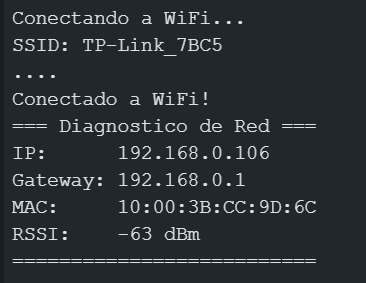
\includegraphics[keepaspectratio]{fotos/Comprobacion_wifi_diagnostico_red.png}}
\caption{Comprobación WiFi y diagnóstico}
\end{figure}

\textbf{Análisis:}

\begin{itemize}
\tightlist
\item
  Confirma asociación correcta a red inalámbrica.
\item
  Permite verificar IP asignada y calidad de enlace (RSSI).
\item
  Es crítica para aislar fallos de conectividad antes de depurar MQTT.
\end{itemize}

\subsubsection{7.2 Diagrama de referencia del
montaje}\label{diagrama-de-referencia-del-montaje}

\textbf{Imagen:} Esquema/diagrama usado en la práctica.

\begin{figure}
\centering
\pandocbounded{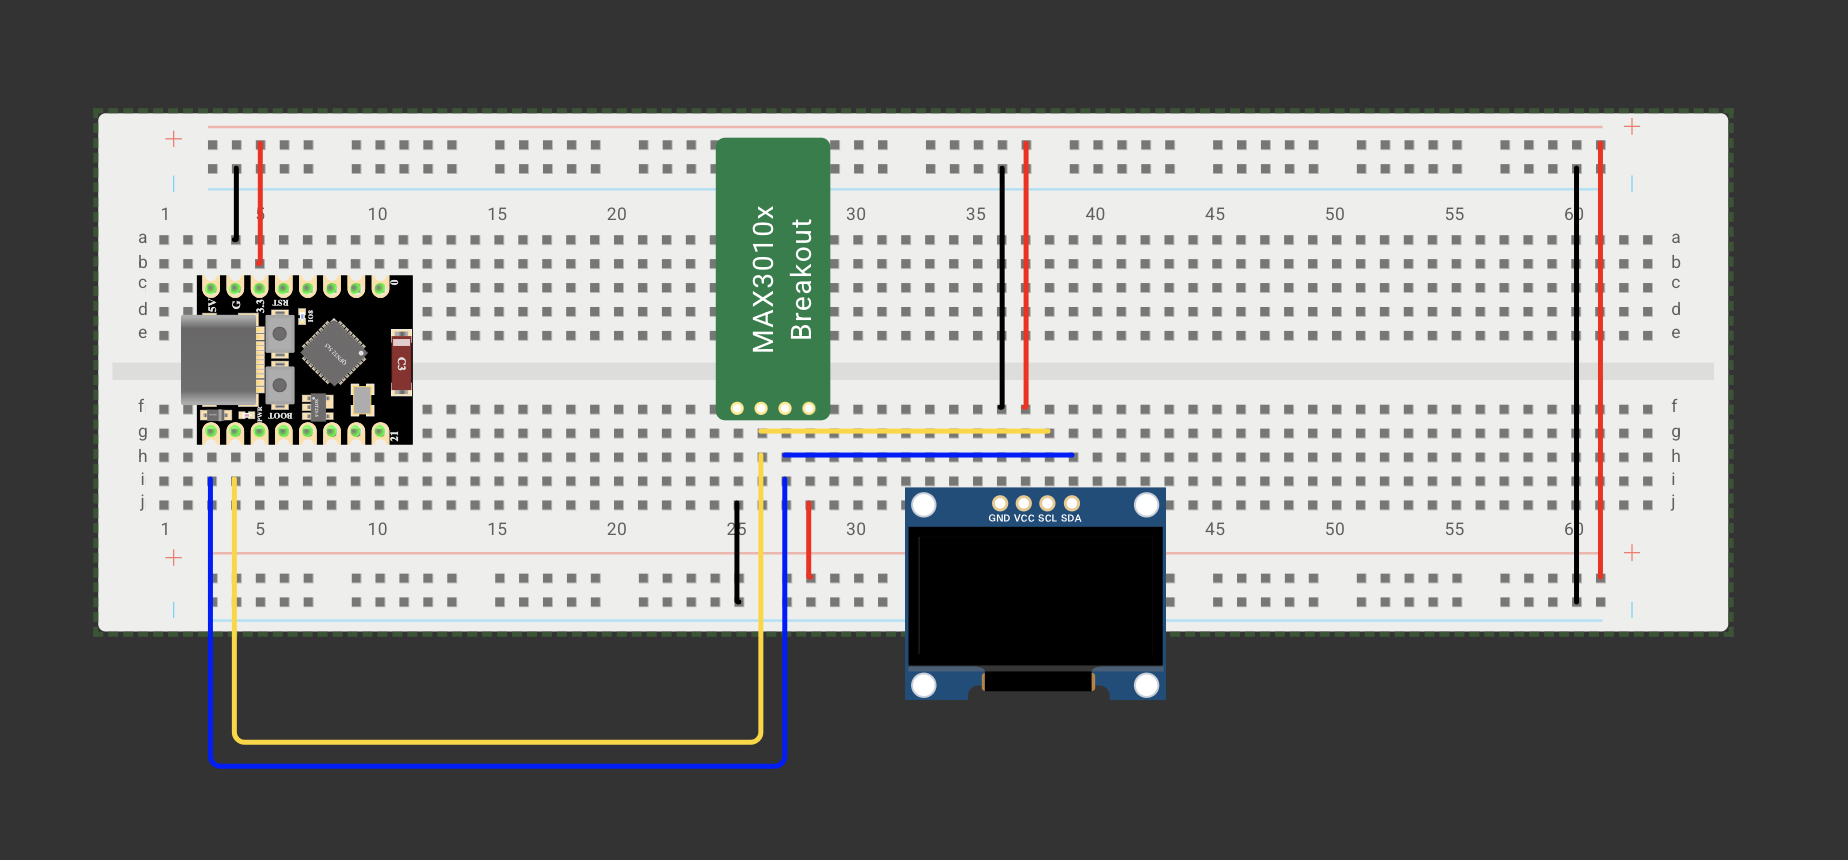
\includegraphics[keepaspectratio]{fotos/diagrama_a_usar.png}}
\caption{Diagrama a usar}
\end{figure}

\textbf{Análisis:}

\begin{itemize}
\tightlist
\item
  Sirve de trazabilidad entre diseño conceptual y montaje efectivo.
\item
  Reduce errores de cableado I2C y alimentación.
\item
  Facilita reproducibilidad para evaluación docente.
\end{itemize}

\subsubsection{7.3 Disparo por regla B
(umbral)}\label{disparo-por-regla-b-umbral}

\textbf{Imagen:} Evidencia de envío por variación significativa.

\begin{figure}
\centering
\pandocbounded{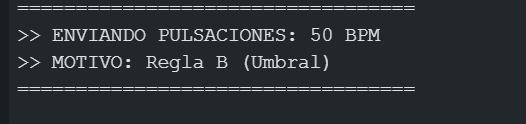
\includegraphics[keepaspectratio]{fotos/motivo_regla_B_umbral.png}}
\caption{Motivo Regla B umbral}
\end{figure}

\textbf{Análisis:}

\begin{itemize}
\tightlist
\item
  Demuestra que el sistema no depende únicamente del temporizador.
\item
  Verifica el comportamiento reactivo ante cambios de pulso.
\item
  Confirma visualmente la etiqueta de motivo de envío.
\end{itemize}

\subsubsection{7.4 Captura de prueba con valor de
pulsaciones}\label{captura-de-prueba-con-valor-de-pulsaciones}

\textbf{Imagen:} Registro de valor de pulsaciones durante
monitorización.

\begin{figure}
\centering
\pandocbounded{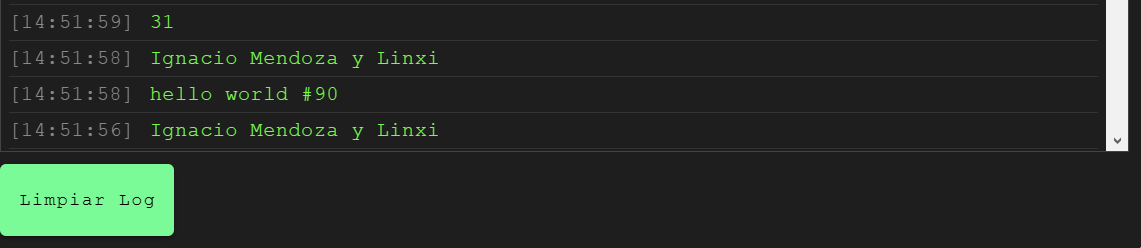
\includegraphics[keepaspectratio]{fotos/prueba_captura_de_pantalla_31_pulsaciones.png}}
\caption{Captura de 31 pulsaciones}
\end{figure}

\textbf{Análisis:}

\begin{itemize}
\tightlist
\item
  Aporta evidencia de adquisición y visualización en tiempo real.
\item
  Es útil para correlacionar lecturas con estado del dedo/sensor.
\item
  Sirve para validar que el pipeline completo está operativo.
\end{itemize}

\subsubsection{7.5 Prueba en entorno de
clase/proyector}\label{prueba-en-entorno-de-claseproyector}

\textbf{Imagen:} Demostración de envío/recepción en infraestructura de
laboratorio.

\begin{figure}
\centering
\pandocbounded{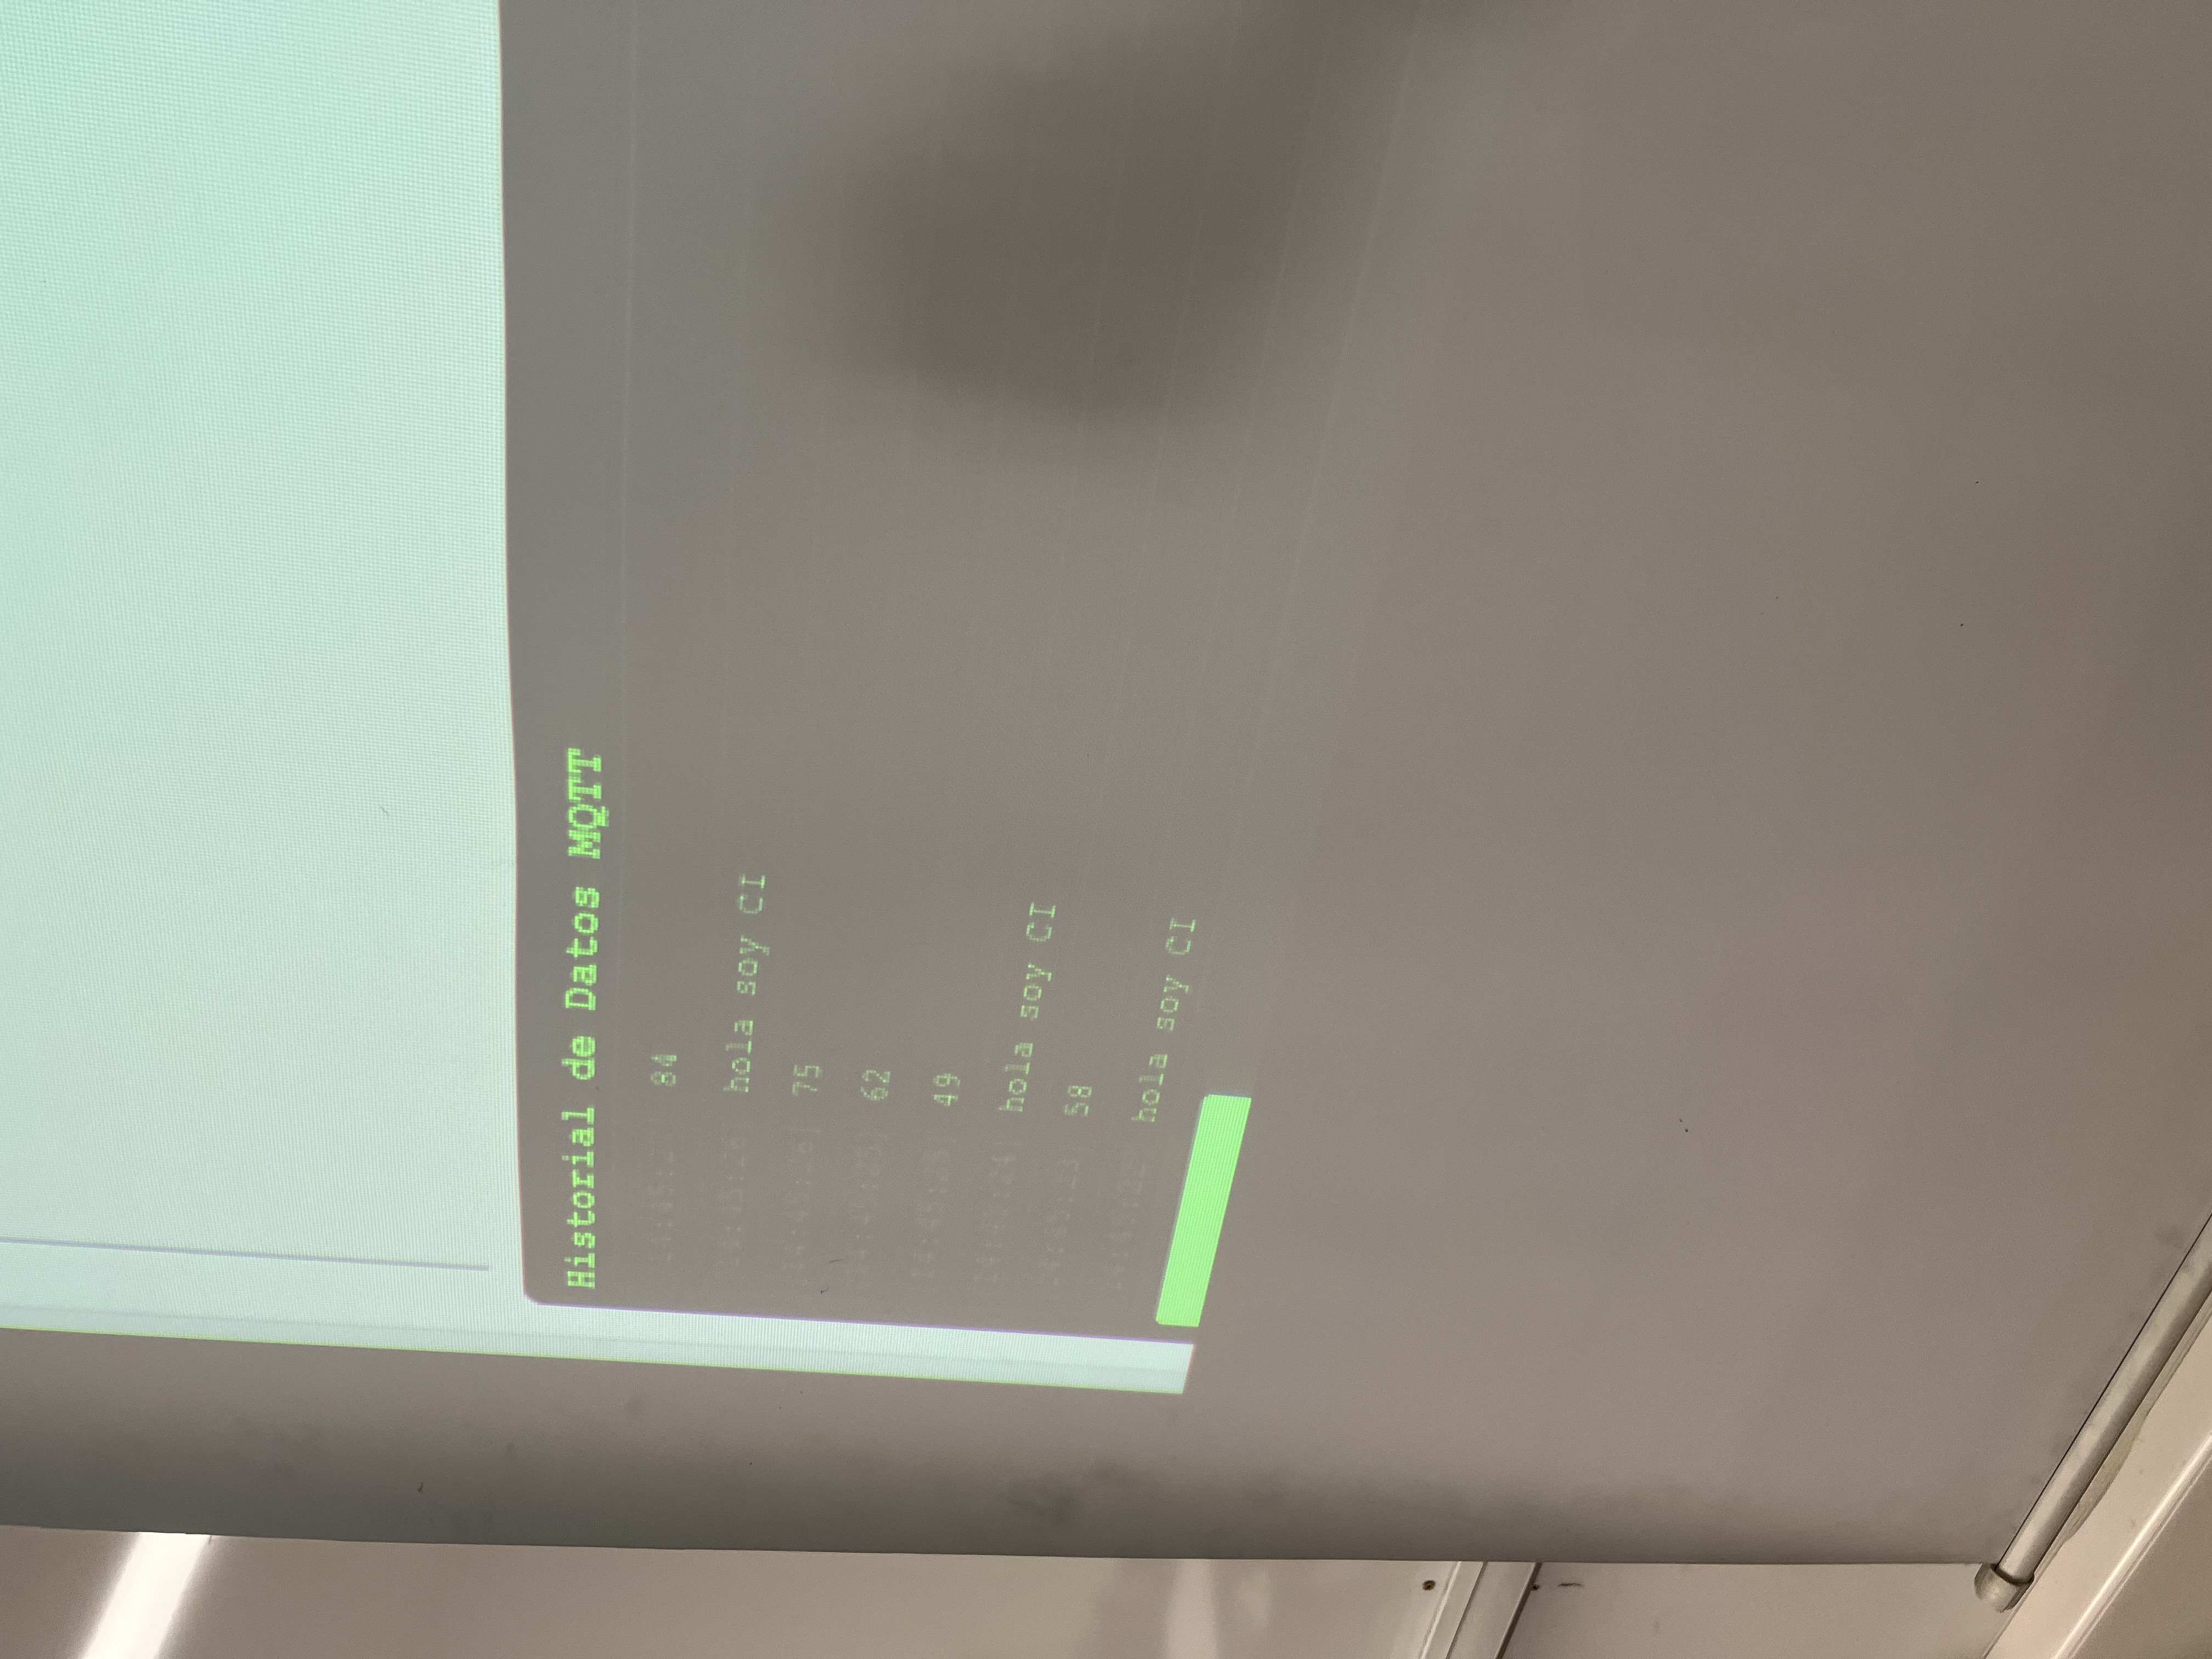
\includegraphics[keepaspectratio]{fotos/prueba_enviando_pulsaciones_proyector_de_clase.jpeg}}
\caption{Prueba enviando pulsaciones en proyector}
\end{figure}

\textbf{Análisis:}

\begin{itemize}
\tightlist
\item
  Evidencia interoperabilidad con el ecosistema de prácticas.
\item
  Demuestra que los datos llegan al panel o cliente de monitorización.
\item
  Refuerza validación de topics y formato de payload.
\end{itemize}

\subsubsection{7.6 Prueba con dedo real sobre el
sensor}\label{prueba-con-dedo-real-sobre-el-sensor}

\textbf{Imagen:} Captura de uso real con contacto físico.

\begin{figure}
\centering
\pandocbounded{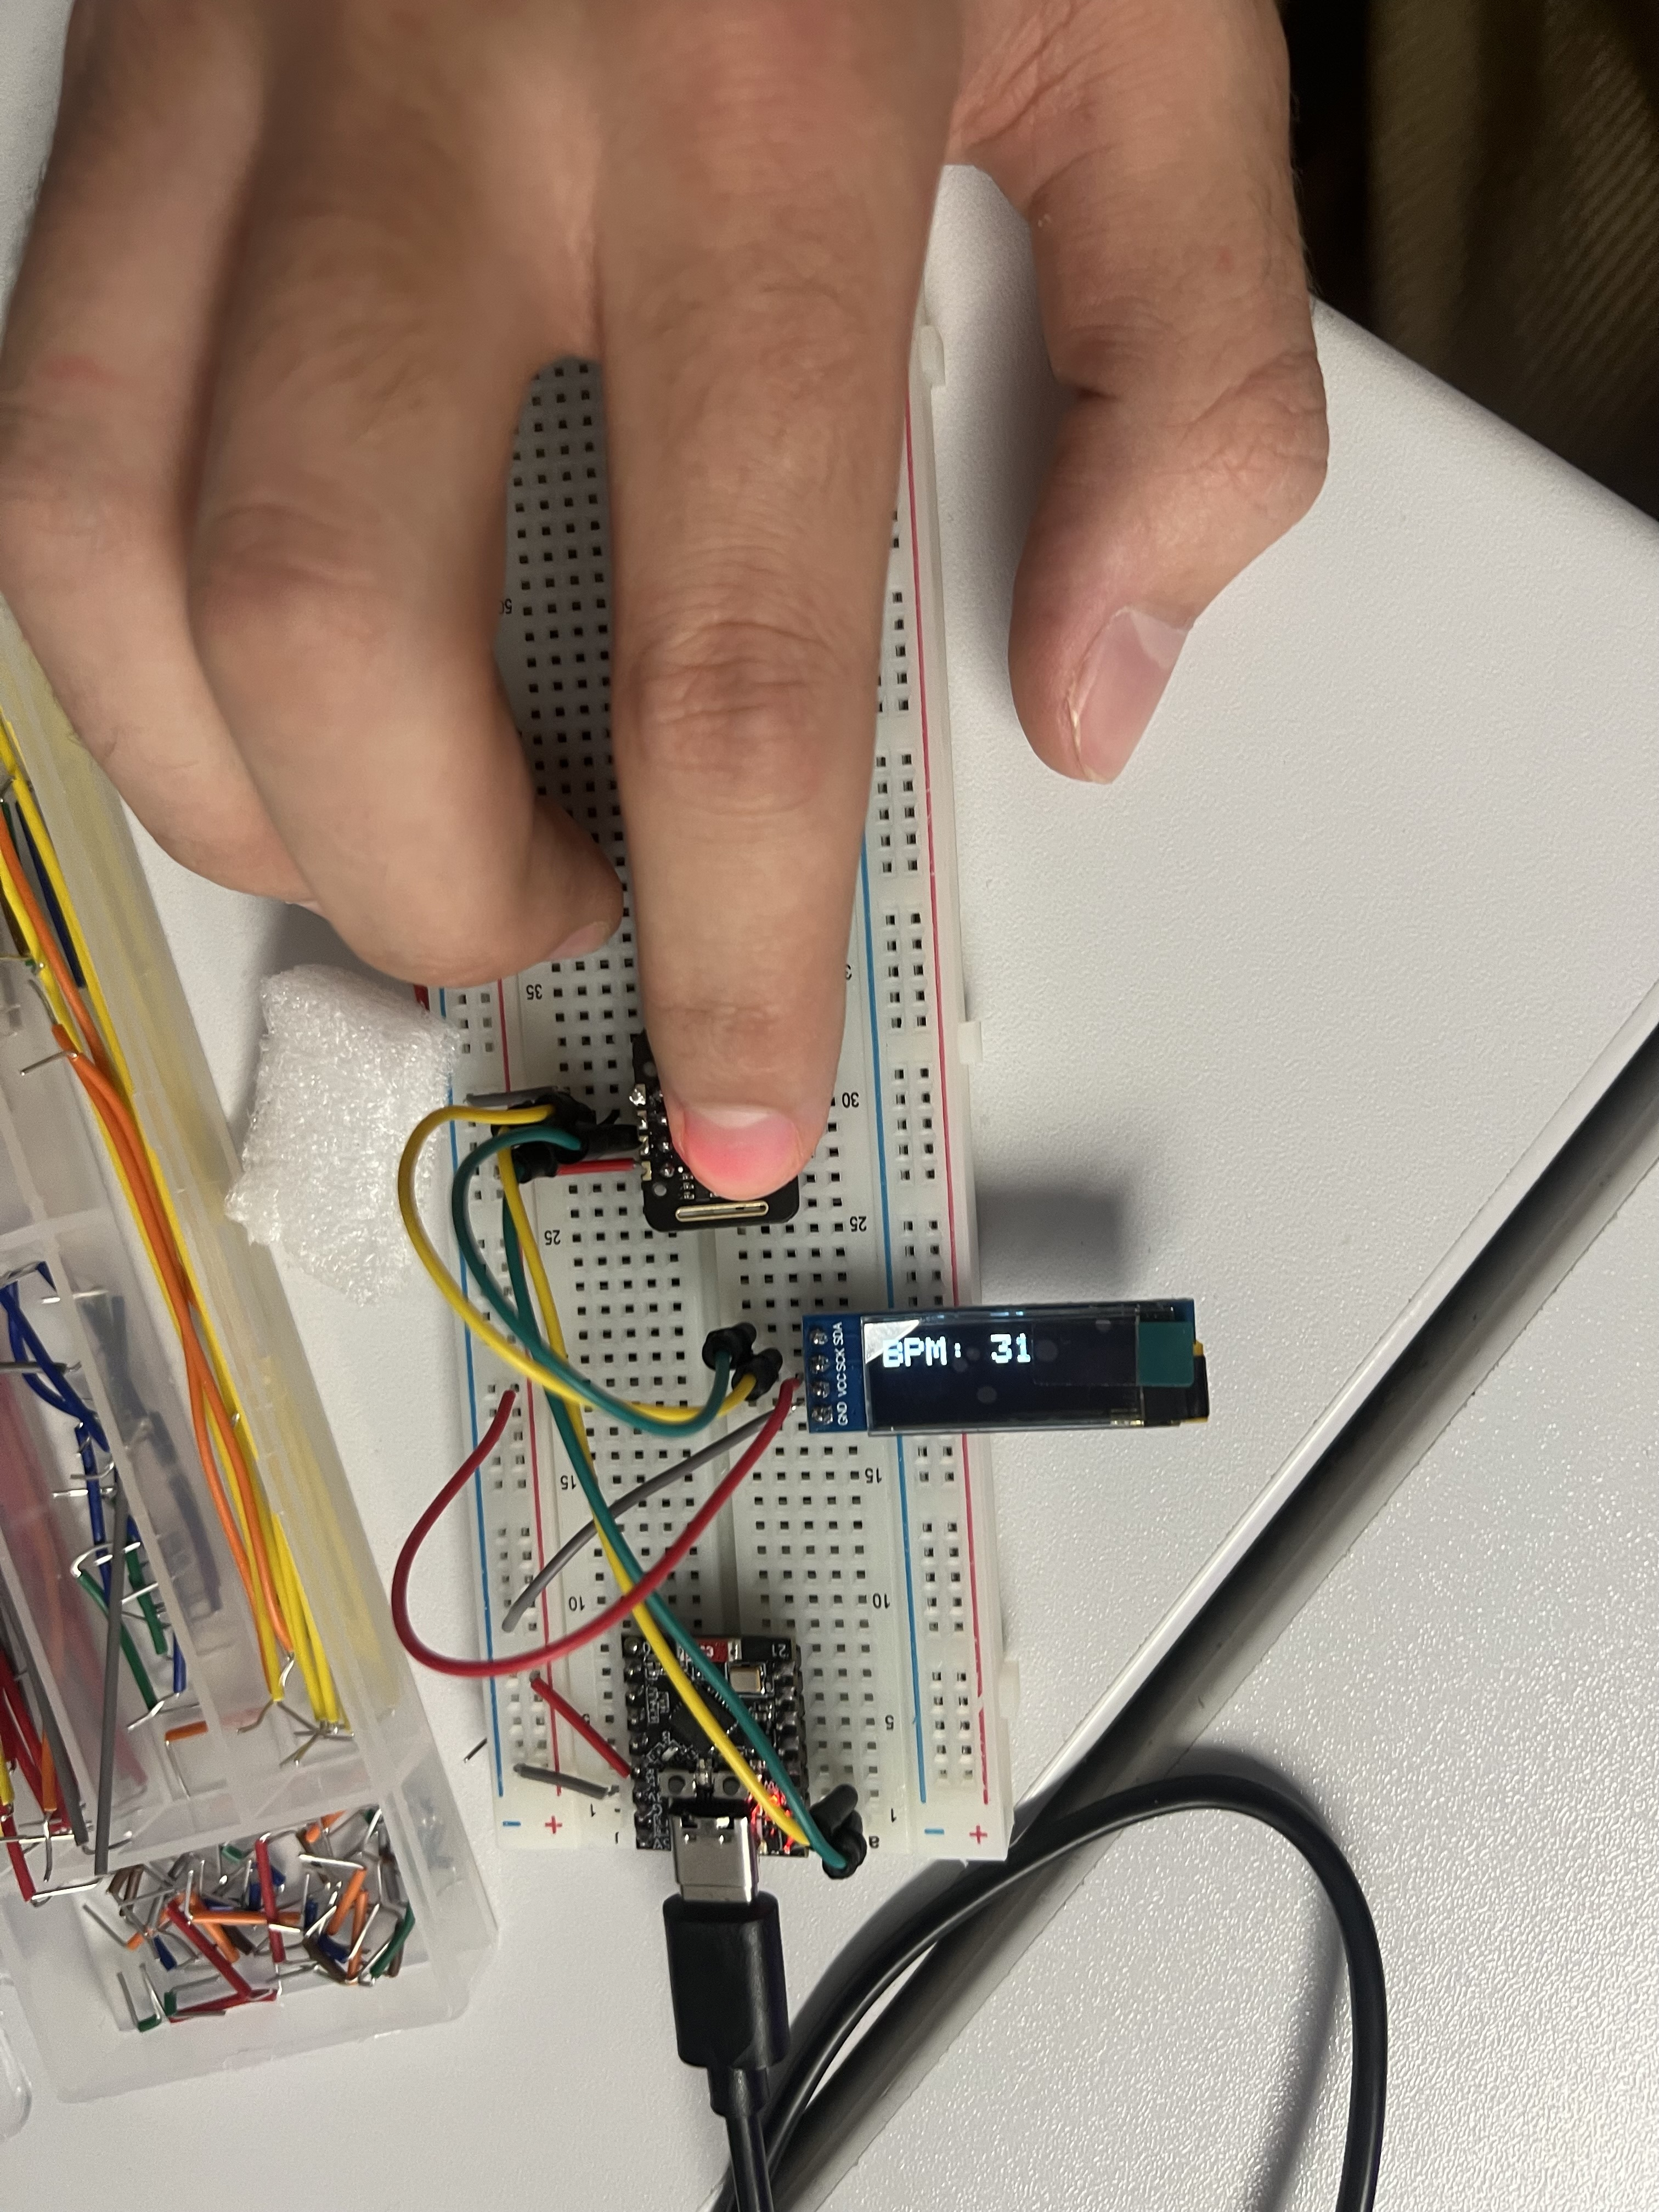
\includegraphics[keepaspectratio]{fotos/pulsaciones_prueba_dedo_real.jpeg}}
\caption{Prueba con dedo real}
\end{figure}

\textbf{Análisis:}

\begin{itemize}
\tightlist
\item
  Verifica comportamiento en condición real de uso.
\item
  Permite observar robustez frente a pequeños movimientos.
\item
  Demuestra que el sistema no se limita a valores simulados.
\end{itemize}

\subsubsection{7.7 Conclusión de resultados
experimentales}\label{conclusiuxf3n-de-resultados-experimentales}

Las evidencias muestran que el sistema:

\begin{itemize}
\tightlist
\item
  Se conecta correctamente por WiFi.
\item
  Publica telemetría MQTT de forma controlada.
\item
  Diferencia motivos de envío según estrategia A/B/C.
\item
  Funciona tanto en ensayo local como en entorno de clase.
\item
  Proporciona feedback inmediato en OLED y monitor serie.
\end{itemize}

    \subsection{8. Trazabilidad de cumplimiento respecto al
enunciado}\label{trazabilidad-de-cumplimiento-respecto-al-enunciado}

\subsubsection{8.1 Parte A: Procesado}\label{parte-a-procesado}

\begin{itemize}
\tightlist
\item
  \textbf{Estabilización de lecturas:} implementada mediante validación
  de latido + media reciente (\texttt{RATE\_SIZE\ =\ 4}).
\item
  \textbf{Downsampling (30 s):} implementado con
  \texttt{sendInterval\ =\ 30000}.
\item
  \textbf{Umbral de cambio (5 BPM):} implementado con
  \texttt{threshold\ =\ 5}.
\item
  \textbf{Alarma BPM \textgreater{} 160 con timeout de 1 min:}
  implementada con \texttt{alarmCondition} y \texttt{lastAlarmTime}.
\item
  \textbf{Mostrar motivo de envío:} implementado y visible en
  OLED/Serial (\texttt{Regla\ A}, \texttt{Regla\ B}, \texttt{Regla\ C}).
\end{itemize}

\subsubsection{8.2 Parte B: Comunicación}\label{parte-b-comunicaciuxf3n}

\begin{itemize}
\tightlist
\item
  \textbf{Credenciales en archivo independiente:}
  \texttt{arduino\_secrets.h} incluido y usado.
\item
  \textbf{Diagnóstico de red del dispositivo:} IP, MAC y RSSI por Serial
  + OLED.
\item
  \textbf{Cliente MQTT operativo:} conexión, publicación y suscripción
  funcionales.
\item
  \textbf{Telemetría en topic de datos:} envío de BPM numérico al topic
  definido.
\item
  \textbf{Recepción de órdenes:} suscripción a topic de órdenes y
  actuación sobre LED.
\end{itemize}

\subsubsection{8.3 Observaciones
técnicas}\label{observaciones-tuxe9cnicas}

\begin{itemize}
\tightlist
\item
  El valor de gateway no se imprime explícitamente en el código actual.
  Si se desea cubrir ese punto al 100\%, basta añadir:
  \texttt{Serial.println(WiFi.gatewayIP());}.
\item
  La parte de filtros SMA/EMA/mediana puede extenderse con
  implementaciones diferenciadas para comparación cuantitativa en
  futuras iteraciones.
\end{itemize}

\subsection{9. Conclusiones y propuestas de
mejora}\label{conclusiones-y-propuestas-de-mejora}

\subsubsection{9.1 Conclusiones}\label{conclusiones}

La práctica cumple el objetivo principal de transformar un prototipo de
lectura biométrica en un \textbf{nodo IoT eficiente}, capaz de:

\begin{itemize}
\tightlist
\item
  Filtrar y decidir localmente.
\item
  Comunicar solo eventos relevantes.
\item
  Mantener telemetría periódica de respaldo.
\item
  Integrarse en flujo MQTT de laboratorio.
\end{itemize}

Desde el punto de vista de ingeniería embebida, el sistema resultante
demuestra un diseño correcto de compromiso entre \textbf{precisión},
\textbf{coste energético} y \textbf{conectividad}.

\subsubsection{9.2 Mejoras recomendadas}\label{mejoras-recomendadas}

\begin{enumerate}
\def\labelenumi{\arabic{enumi}.}
\tightlist
\item
  Separar módulos en archivos (\texttt{sensor.cpp}, \texttt{mqtt.cpp},
  \texttt{display.cpp}) para mejorar mantenibilidad.
\item
  Añadir comparación explícita de filtros (SMA/EMA/mediana) con métricas
  de varianza y latencia.
\item
  Incorporar histéresis de alarma avanzada (umbral alto/umbral bajo)
  además del timeout.
\item
  Migrar a MQTT con TLS en entornos no académicos.
\item
  Persistir eventos críticos en memoria local por si se pierde
  conectividad.
\end{enumerate}

\begin{center}\rule{0.5\linewidth}{0.5pt}\end{center}

\subsection{Anexo: comando de despliegue opcional de broker
local}\label{anexo-comando-de-despliegue-opcional-de-broker-local}

Si se opta por alternativa local con Docker (según enunciado):

\begin{Shaded}
\begin{Highlighting}[]
\NormalTok{docker}\OperatorTok{{-}}\NormalTok{compose up }\OperatorTok{{-}}\NormalTok{d}
\end{Highlighting}
\end{Shaded}

Después se puede acceder a paneles como \texttt{http://127.0.0.1:1880/}
y configurar el ESP32 apuntando a la IP local del equipo host.


    % Add a bibliography block to the postdoc
    
    
    
\end{document}
